\documentclass[a4paper,11pt]{article}
%\hyphenpenalty 10000
\usepackage[utf8]{inputenc}
%\usepackage[T1]{fontenc}
\usepackage{amsmath,amssymb}
\usepackage[english,french]{babel}
\usepackage[pdftex]{graphicx}
%\usepackage[options]{mcode}
\usepackage{textcomp}
\usepackage{array}
\usepackage{subfig}
\usepackage[left=2cm, right=1cm, bottom=2cm, top=2cm]{geometry}
\usepackage{float}
\usepackage{multicol}
\usepackage{tabularx}
\usepackage{fancybox}



\usepackage{color} % gestion de différentes couleurs

\definecolor{linkcolor}{rgb}{0,0,0.6} % définition de la couleur des liens pdf
\usepackage[ pdftex,colorlinks=true,
pdfstartview=FitV,
linkcolor= linkcolor,
citecolor= linkcolor,
urlcolor= linkcolor,
hyperindex=true,
hyperfigures=false]
{hyperref} % fichiers pdf 'intelligents', avec des liens entre les références, etc.

\usepackage{fancyhdr} % entêtes et pieds de pages personnalisés 
\pagestyle{fancy}
\fancyhead[L]{\scriptsize \textsc{Etude théorique de la translocation de
biomolécules à travers un nanopore}}
\fancyhead[R]{\scriptsize \textsc{Menais Timothée}}
\fancyfoot[C]{ \thepage} 

\begin{document}



% Pour faciliter la mise en forme de la page du titre, on supprime l'indentation automatique en début de paragraphe
\setlength{\parindent}{0pt}

% Pas d'en-tête ni de pied pour la première page
\thispagestyle{empty}

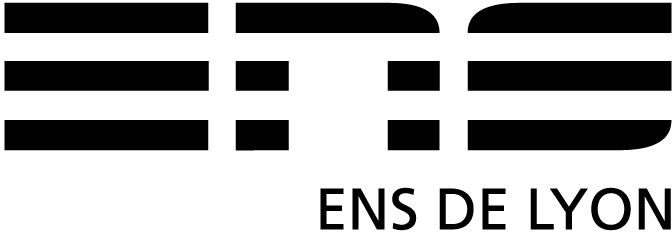
\includegraphics[height=1.5cm]{ens.png} \hfill 
\includegraphics[height=2cm]{cea2.png} \hfill 
\includegraphics[height=2cm]{phelma.jpg}

\vspace{0.5cm}

\begin{tabularx}{\textwidth}{@{} l X l @{} }
{\sc Master d'ouverture - Master  2R EP} & & Rapport de stage 2012 \\
{\it ENS de Lyon - Grenoble INP, PHELMA} & & Menais Timothée \\

\end{tabularx}

\begin{center}

\vspace{1.5cm}

\rule[11pt]{5cm}{0.5pt}

\textbf{\huge Etude théorique de la translocation de
biomolécules à travers un nanopore}

\rule{5cm}{0.5pt}

\vspace{1.5cm}

\parbox{15cm}{\small
\textbf{Abstract} : \it Stage de M2, Timothée Menais, 2011-2012.

\vspace{0.5cm}
\rm Durant mon stage, j'ai étudié d'un point de vu analytique et numérique la translocation (passage) de biomolécules (principalement de l'ADN simple brin) à travers un nanopore de graphène, au sein du Groupe Théorie, SPrAM, INAC du CEA de Grenoble. Intéressante d'un point de vue fondamental, cette étude peut également avoir des retombées importantes pour la compréhension de phénomènes biologiques et des applications techniques notamment pour le séquençage de génomes. Des outils théoriques de physique statistique et numériques de dynamique moléculaire ont été mis en œuvre afin de comprendre le rôle et l'importance de la structure du polymère et des forces appliquées sur le temps nécessaire à la translocation. De récentes expériences utilisant des pores dans une mono-couche de graphène ont produit des résultats encourageants qui nous poussent à concentrer notre étude sur la compréhension et la modélisation de ces nouveaux pores. Notre modèle original, suffisamment détaillé pour reproduire des comportements de l'ADN simple brin, mais suffisamment simple pour permettre de mettre en œuvre des études statistiques, nous a permis d'évaluer les lois de puissances régissant le temps de translocation, pour un nanopore large, ainsi que pour un nanopore étroit.
} %fin de la commande \parbox du résumé


\vspace{0.5cm}

\parbox{15cm}{
\textbf{Mots clés : \it ADN, Graphène, Dynamique moléculaire, Physique statistique.} }%fin de la commande \parbox des mots clefs

\vspace{0.5cm}

\parbox{15cm}{
Stage encadré par :

{\bf Dr Arnaud Buhot }

\href{mailto:	arnaud.buhot@cea.fr }{\tt 	arnaud.buhot@cea.fr }  / tel: ++33 438 78 38 68

%{\bf Dr Ulrich Keyser}

%\href{mailto:	ufk20@cam.ac.uk}{\tt 	ufk20@cam.ac.uk} / tel: +44 (0)1223 337272

Groupe Théorie

Structures et Propriétés d'Architectures Moléculaires

Institut Nanoscience et Cryogénie
{\it 

17 rue des Martyrs
38054 Grenoble cedex 9
France}

\url{http://inac.cea.fr/spram/Phocea/Vie_des_labos/Ast/ast_groupe.php?id_groupe=397}
} %fin de la commande \parbox encadrant / laboratoire d'accueil

\vspace{1cm}



\includegraphics[height=1.8cm]{spram.jpg} \hspace{0.3cm}

\includegraphics[height=1.8cm]{inac.jpg}

\end{center}
\selectlanguage{french}

\begin{flushright}
\today
\end{flushright}

\vfill
\hfill 

% Pas d'entête ni de pied pour la page de sommaire



\setlength{\parindent}{10pt}

\section*{Remerciements}

Je tiens tout particulièrement à remercier mes encadrants, Arnaud et Stefano, qui ont su me transmettre leur passion de la physique des polymères et de la dynamique moléculaire à travers une pédagogie exemplaire. J'ai bénéficié à la fois de leur confiance et de leur présence. J'ai ainsi pu être indépendant et faire mes propres erreurs, mais leurs conseils m'ont maintes fois sorti de l'impasse. Tant sur le plan scientifique que sur le plan humain, ils ont permis de faire de ce stage une très bonne expérience.

J'ai aussi grandement apprécié les repas du midi pris en compagnie de chercheurs de toutes origines, leurs points de vue d'Inde, d’Asie et d'Amérique latine offrent un éclairage nouveau sur le monde et les sciences. 

\section*{Introduction}


La translocation (passage) de biomolécules à travers un nanopore est un domaine scientifique très actif, tant sur le plan expérimental que sur le plan théorique. Ceci est principalement dû aux applications potentielles en biotechnologies et en médecine, notamment le séquençage rapide et économique envisagé lors de la translocation de brins d'ADN. L'aspect appliqué est important mais ce problème soulève aussi des questions fondamentales très intéres$\-$santes sur le comportement de polymères lorsqu'ils sont confinés.\\

De récentes expériences de translocation mettent en œuvre des nanopores creusés dans des couches monoatomique de graphène. Le graphène, isolé pour la première fois en 2004, est un cristal aromatique bidimensionnel de carbone dont l'empilement de plusieurs plans forme le graphite. Ces expériences contournent les problèmes d'épaisseur inhérents aux autres types de pores, mais apportent d'autres difficultés.\\

Au cours du présent travail, nous avons modélisé la translocation d'un polymère à travers un nanopore de graphène en utilisant un modèle gros grain pour notre polymère, analogue sur de nombreux points à l'ADN. Des éléments de physique statistique et l'utilisation de la dynamique moléculaire ont permis de vérifier des lois d'échelles. Notre approche original, à mi chemin entre le modèle détaillé et le modèle simple idéal, nous a permis de déterminer les exposants critiques. Ces exposants sont caractéristiques des lois de puissances suivies par le temps de translocation en fonction de la taille du polymère et de la force qu'on lui applique.\\

Ce rapport s'articule autour d'un premier chapitre présentant les systèmes impliqués, d'un second chapitre portant sur la modélisation numérique du problème, et d'un dernier chapitre mettant en parallèle les résultats théoriques et numériques.



\tableofcontents



\newpage 

\section{Systèmes étudiés}
Dans un premier temps, nous allons décrire les systèmes et concepts impliqués dans notre étude.


\subsection{L'ADN}

Les bio-polymères, et notamment l'ADN, sont les polymères qui constituent le vivant. Ils interviennent dans de nombreux processus clés en biologie. La modélisation de ces polymères permet de comprendre ces processus.\\

Dans notre étude nous avons utilisé un modèle proche de l'ADN. L'ADN (avec l'ARN) est le support de l'information génétique du vivant. Il se trouve dans les cellules, contenu généralement dans le noyau. C'est un bio-polymère constitué d'une séquence de quatre monomères différents. Ces monomères, appelés nucléotides sont constitués de phosphate, de sucre et d'une des bases azotées, seul élément distinct entre nucléotides: l'adénine, la cytosine, la guanine et la thymine. 

\begin{figure}[H]
\begin{center}
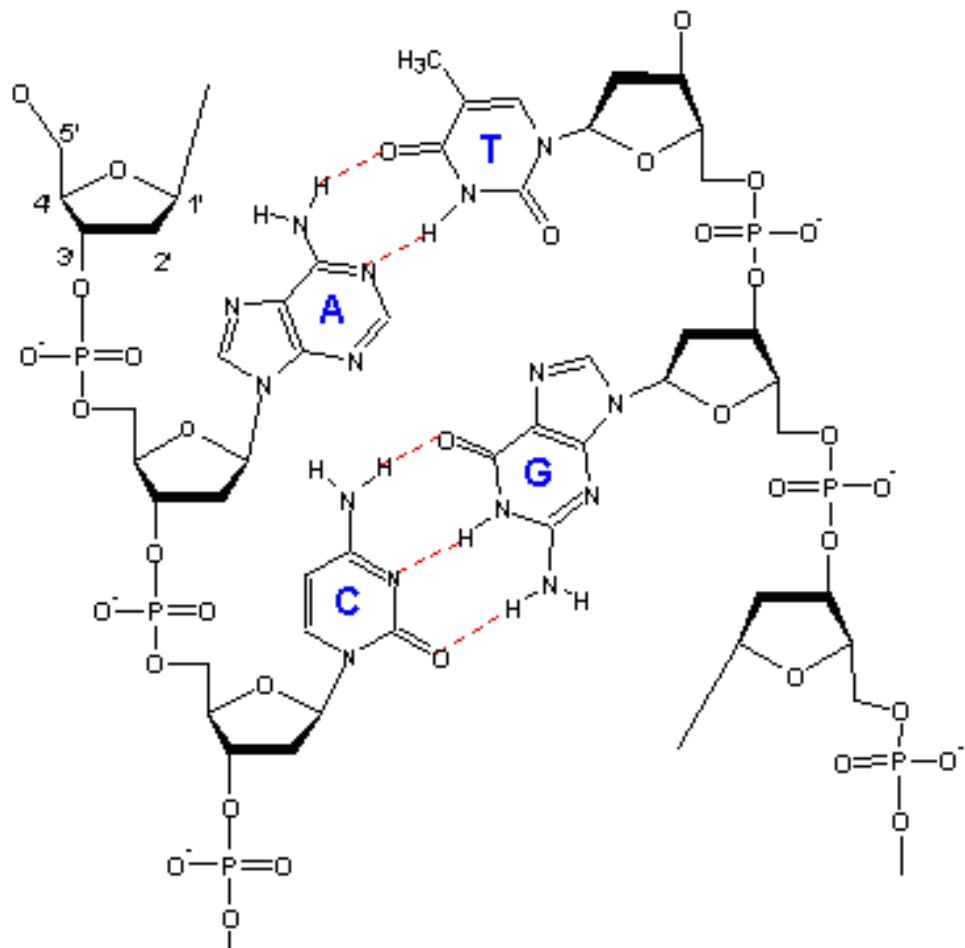
\includegraphics[width=0.58\textwidth]{adn.jpg}

\caption{Structure chimique de l'ADN. Le squelette est composé d'une succession de phosphates et de sucres liés entre eux, chacun des sucres est de plus lié à une base azotée. Les bases azotées peuvent interagir par liaisons hydrogènes et interactions orbitalaires.}
\label{adn}
\end{center}
\end{figure}

La structure chimique de l'ADN est aujourd'hui parfaitement connue (Figure \ref{adn}), la nature des liaisons et interactions ne sont plus mystérieuses. Toutefois, son comportement, dépendant de la séquence, et l'unicité du code génétique de chaque individu,  font de la compréhension de l'ADN et de son séquençage des enjeux majeurs. Ces enjeux justifient de mettre en œuvre des modèles et simulations afin de comprendre les mécanismes essentiels du vivant associés à l'ADN.\\

Ce bio-polymère présente une structure très complexe qui demande des ressources numériques très importantes si l'on souhaite la modéliser entièrement au niveau atomique. Nous souhaitons effectuer une étude statistique sur de nombreuses simulations, ce qui implique de baisser le niveau de résolution du modèle en ne gardant que les éléments cruciaux.

  

\subsection{La translocation de polymères}
Très récemment, le développement des expériences sur molécule unique (permises par des technologie novatrices tel les pinces optiques et pointes AFM \cite{keyser}) ont permis de s'affranchir des moyennes macroscopiques classiques et d'investiguer en profondeur les processus moléculaires clés en biologie.\\

Parmi les phénomènes dont l'étude est dorénavant possible, figure la translocation. La translocation d'un polymère est son passage par un pore reliant deux compartiments séparés par une membrane. La compréhension de ce processus est essentielle pour la biologie. En effet, la translocation de l'ARN entre le noyau et la cellule est primordiale chez l'homme. C'est aussi le mécanisme utilisé par de nombreux virus pour infecter des cellules avec leur ADN. Enfin sa maitrise permettrait d'ouvrir de nombreuses voies pour la biotechnologie, notamment dans le domaine de la thérapie génique.\\

 Lors de la translocation, la molécule passe d'un coté appelé cis à l'autre appelé trans en deux étapes. La première étape consiste en ce qu'une extrémité de la chaîne atteigne l'entrée du pore. La probabilité d'accéder au pore et le temps caractéristique qui lui est associé ont déjà été estimés analytiquement \cite{milchev}. La deuxième étape, lorsque le pore est occupé, a retenu notre attention (voir Figure \ref{transloc}). \\

\begin{figure}[H]
\begin{center}
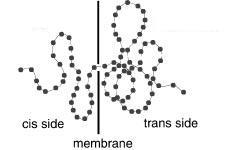
\includegraphics[width=0.37\textwidth]{transloc.jpg}

\caption{Un polymère effectue une translocation d'un coté de la membrane appelé cis vers l'autre appelé trans. Le temps pendant lequel le pore est occupé est appelé temps de translocation (illustration réf: \cite{sung}).}
\label{transloc}
\end{center}
\end{figure}



Le temps pendant lequel le pore est occupé, appelé temps de translocation ($\tau$) est très important puisqu'il représente dans beaucoup de cas la seule mesure expérimentale accessible. Ce temps de translocation va dépendre de plusieurs paramètres notamment la longueur du polymère, l'application éventuelle d'une force (translocation biaisée ou libre), la façon dont elle est appliquée... Nous reviendrons sur ces facteurs dans la partie théorie.\\

 Une idée directrice des expériences au cours de la dernière décennie est la mesure du courant ionique à travers le pore au cours de la translocation \cite{holesedge}. Ce courant est caractéristique de l'élément en cours de translocation. Expérimentalement, il a déjà été démontré que la mesure de ce courant de translocation permet de détecter et d'identifier des protéines. Il permet également de déterminer leurs différentes conformations ainsi que celles de l'ADN lorsqu'ils sont au sein du pore.\\
 
Le courant est fortement modifié au cours de ces expériences, cependant la limite de résolution en courant nécessaire afin de séquencer est atteinte. La première source de limitation est temporelle: la translocation a généralement lieu trop rapidement pour que les variations de courant soient observables. La seconde est spatiale. En effet les pores utilisés jusqu'à présent sont bien trop épais et plusieurs dizaines de bases sont simultanément au sein du pore lors de la translocation, ce qui rend très difficile de distinguer les unes des autres les nombreuses séquences possibles.
 
 






\subsection{Le graphène}

Comme nous l'avons déjà souligné, le principal obstacle au séquençage par analyse du courant de translocation est l'épaisseur trop importante du pore qui ne permet pas de distinguer les multiples combinaisons de séquences possibles. Ce problème pourrait bien être résolu par l'utilisation du graphène ( le lecteur intéressé trouvera en annexe une page illustrant les pores classiques utilisés jusqu'à maintenant).\\

Isolé pour la première fois en 2004, le graphène est un cristal bidimensionnel de carbone \cite{graph}. L'empilement de plusieurs couches monoatomiques de graphène forme le graphite. Comme le montre la Figure \ref{orbit}, les carbones forment un maillage hexagonal de paramètre de maille d= 0.142 $nm$, les électrons délocalisés sur l'ensemble des orbitales $\pi$ de ce plan le rendent aromatique. L'occupation de ces orbitales $\pi$ est l'origine de propriétés intéressantes du graphène. Les électrons $\pi$ octroient au graphène une importante conductivité. Les interactions orbitalaires (stacking) maintiennent une cohésion entre les différents plans. La distance inter-planaire dans le graphite, 0.335 $nm$, est plus importante que la distance inter-atomique dans le plan, cela est dû à la géométrie plus étendue perpendiculairement au plan des orbitales $\pi$.

\begin{figure}[H]
\begin{center}
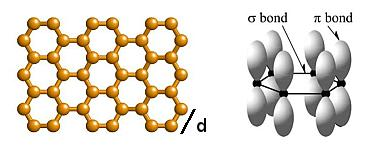
\includegraphics[width=0.55\textwidth]{orbitals2.jpg} 
\caption{Structure cristallographique et orbitales $\pi$ du graphène.}
\label{orbit}
\end{center}
\end{figure}
 
Expérimentalement, il a été vérifié que la translocation d'ADN à travers un nanopore creusé dans le graphène est possible \cite{dnatrans}. C'est une porte ouverte à de nombreuses autres expériences. La finesse de la couche monoatomique de graphène entraine cependant des différences singulières par rapport aux pores utilisés précédemment. En effet, l'épaisseur importante d'un pore impose une certaine rigidité à ce dernier. Ce n'est plus le cas lors de l'utilisation de pores creusés dans le plan de graphène, qui est déformable et présente des propriétés vibrationnelles complexes, comme l'illustre la Figure \ref{vib}.


\begin{figure}[H]
\begin{center}
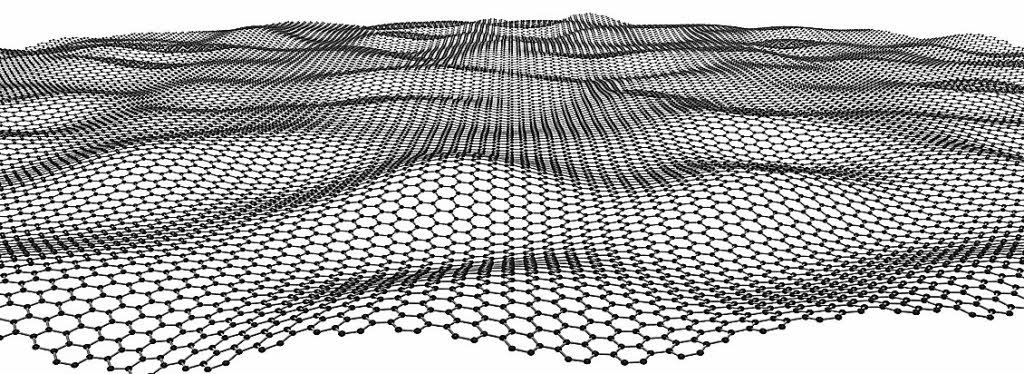
\includegraphics[width=0.8\textwidth]{vib.jpg} 
\caption{La couche monoatomique de graphène, flexible, présente des propriétés vibrationnelles complexes.}
\label{vib}
\end{center}
\end{figure}

Dans ce nouveau cadre expérimental, les futurs expériences pourraient être complétées et interprétées par une étude théorique et numérique de l'influence des propriétés uniques du graphène sur la translocation.


\newpage
\section{Méthodes numériques de la dynamique moléculaire et modèle}



Dans le cadre de mon projet, nous avons envisagé une approche assez différente des simulations classiques sur réseau avec maillage comme c'est souvent le cas en mécanique des fluides ou dans certains travaux sur les polymères \cite{these}. Nous avons décidé de modéliser hors réseau les différentes parties du polymère en regroupant plusieurs atomes voisins dans un centre d'interaction effectif dit gros grain. Les gros grains interagissent entre eux par le biais de forces conservatives issues de potentiels adaptés. En intégrant numériquement les équations du mouvement associées, on est capable de produire plusieurs trajectoires pour le système. C'est ce qu'on appelle faire de la dynamique moléculaire.\\

Basé sur des données expérimentales, le modèle de Margaret C Linak et collaborateurs \cite{jchem} reproduit correctement le comportement de l'ADN simple brin. Nous avons choisi de nous en inspirer fortement en ce qui concerne la modélisation du polymère. Le paragraphe suivant décrit ce modèle.

\subsection{Exemple de modèle gros grains}

Afin de créer un modèle numérique fiable et robuste de l'ADN, il convient de décomposer chaque monomère en sous-systèmes. Margaret C Linak et collaborateurs \cite{jchem} ont choisi de décomposer chaque nucléotide en trois grains: le sucre, le phosphate et la base azotée (Figure \ref{dnamod}).
\begin{figure}[H]
\begin{center}
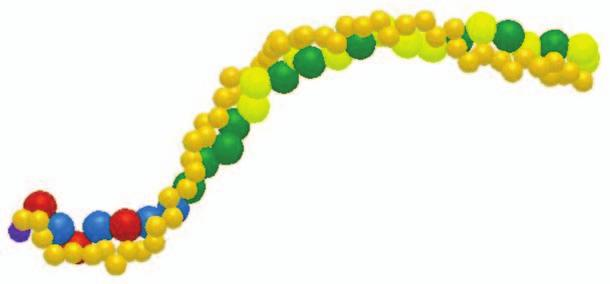
\includegraphics[width=0.32\textwidth]{dnamod.jpg}

\caption{Chaîne de nucléotides avec trois composants: sucres, phosphates et bases azotées \cite{jchem}.}
\label{dnamod}
\end{center}
\end{figure}

Une fois ce découpage préparé, l'étape suivante consiste à définir les potentiels d'interaction entre les différents grains. Plusieurs types de potentiels sont définis à partir d'étalons de distance ($\sigma$ et $R_0$) et d'énergie ($\epsilon$) qui traduisent les propriétés physiques du polymère. A partir de ces valeurs on peut créer des échelles a-dimensionnées de temps, température, viscosité, force... On parle d'unités de Lennard-Jones. La Figure \ref{moldyn} récapitule les potentiels utilisés.

\subsubsection*{Les interactions stériques:}

Il s'agit des interactions de type volume exclu, modélisées par un potentiel de Lennard-Jones:

\begin{eqnarray}
U_{EV}(r_{ij})= 4\epsilon \left[\left(\frac{\sigma}{r_{ij}}\right)^{12}-\left(\frac{\sigma}{r_{ij}}\right)^{6}\right] + \epsilon \text{ }, \text{ } U_{EV}(r_{ij})=0 \text{ pour }  r_{ij}> 2.25 \sigma
\end{eqnarray}

$r_{ij}$ étant la distance entre les billes i et j, ce potentiel empêche l'interpénétration à faible distance et est équivalent aux interactions de Van der Waals à longues distances. Un $\sigma$ moyen est utilisé pour le contact de grains de tailles différentes.\\

Ainsi que des liaisons covalentes, modélisées par un potentiel anharmonique de type FENE (Finitely Extensible Nonlinear Elastic) bonds:
\begin{eqnarray}
U_{MH}(r_{ij})= -15\epsilon \left(\frac{R_0}{\sigma}\right)^2\text{ } \ln\left[1-\left(\frac{r_{ij}}{R_0}\right)^2\right]
\end{eqnarray}


Un développement limité montre le comportement harmonique à faible distance et le logarithme impose une extension maximale de la liaison. Le potentiel FENE représentant la contribution attractive de la liaison covalente est utilisé en complément du potentiel de Lennard-Jones, répulsif à courte distance. Il en résulte une position d'équilibre très stable qui est caractéristique de la longueur de la liaison. Les potentiels des interactions stériques sont tracés sur la Figure \ref{moldyn}.


\subsubsection*{Autres interactions:}

La rigidité angulaire du squelette du polymère implique un potentiel faisant  intervenir l'angle formé par trois grains successifs de la chaîne. Les bases interagissent entre elles en formant des liaisons hydrogènes, ou par interactions orbitalaires entre cycles aromatiques.\\

 C'est la combinaison de la torsion avec les interactions orbitalaires pour l'ADN simple brin, qui permet le maintient d'une structure hélicoïdale. Dans l'ADN double brin, deux structures hélicoïdales en vis-à-vis sont renforcées par les liaisons hydrogènes. Un schéma représentant les divers types d'interactions modélisées est disponible en Figure \ref{moldyn}.\\



\begin{figure}[H]
\begin{center}
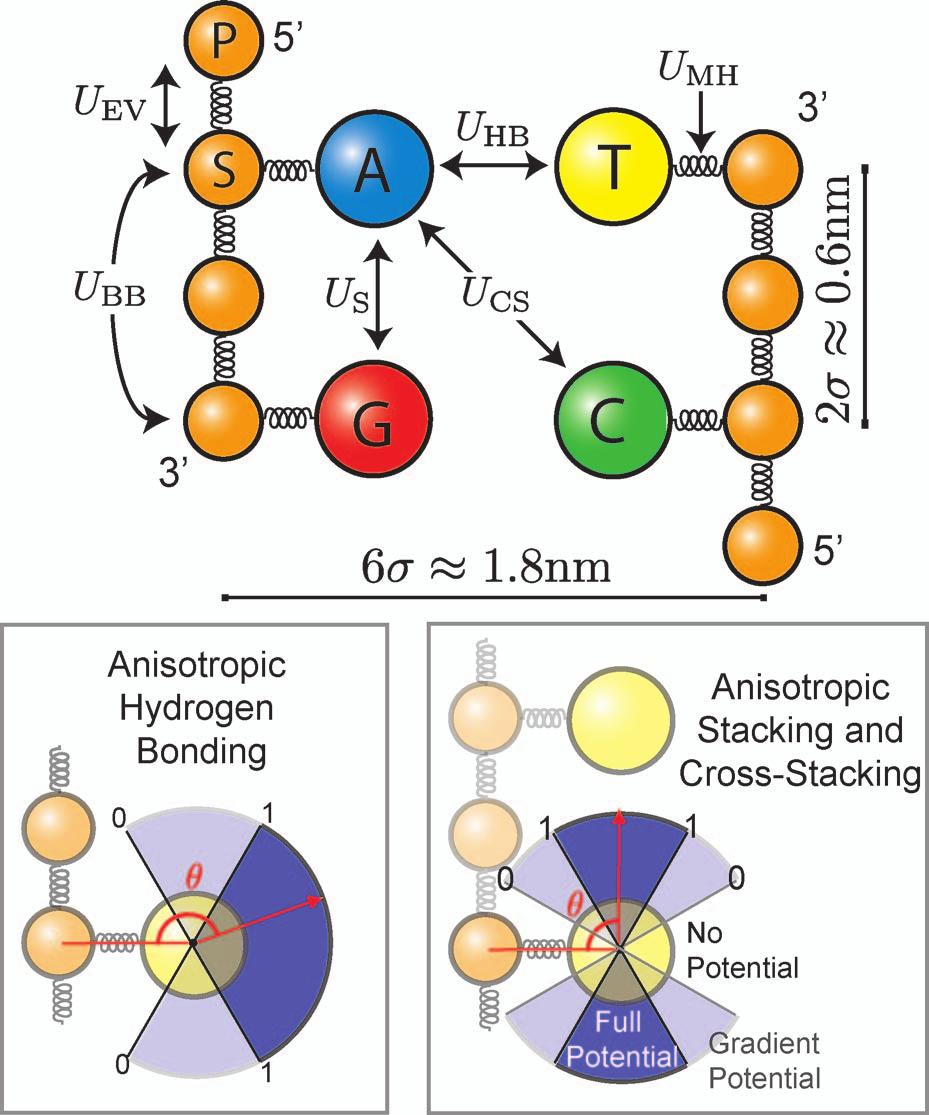
\includegraphics[width=0.5\textwidth]{moldyn.jpg}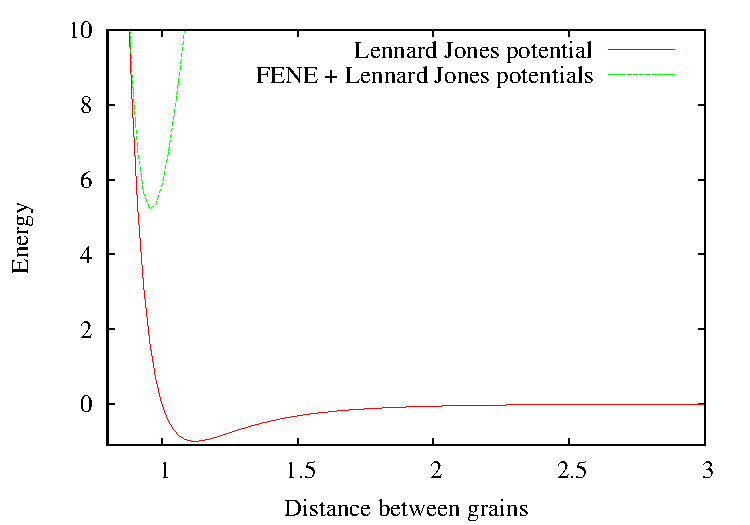
\includegraphics[width=0.54\textwidth]{potentials.pdf}


\caption{A gauche: les différentes interactions modélisées dans le modèle de Margaret C Linak et collaborateurs \cite{jchem}. A droite: la valeur des potentiels stériques (en unité de $\epsilon$) en fonction de la distance entre les grains (en unités de $\sigma$), le potentiel combiné a été abaissé pour plus de clarté. La partie fortement répulsive du potentiel de Lennard-Jones empêche l'interpénétration des grains, la partie faiblement attractive représente les intéractions de Wan Der Waals. La position d'équilibre de deux grains liés est autour de $\sigma$ dans un potentiel localement harmonique.}
\label{moldyn}
\end{center}
\end{figure}

Le modèle de Margaret C Linak et collaborateurs \cite{jchem} répond efficacement aux problématiques qu'ils se sont fixés, cependant il n'est pas complétement adapté aux nôtres. Nous voulons comparer nos résultats à des prédictions théoriques de physique statistique, ce qui implique l'analyse d'un nombre assez important d'événements, et donc des ressources numériques très sollicitées.\\

\subsection{Notre modèle}

Lors de l'élaboration de notre modèle, nous avons dû considérer, la façon de représenter le polymère, comment modéliser le plan de graphène, ainsi que la manière dont ils vont interagir l'un avec l'autre.

\subsubsection*{Le polymère:}

Le modèle présenté précédemment est trop complet pour que nous puissions l'exploiter et générer des données statistiquement significatives. Notre intérêt se porte principalement sur les interactions de contact avec le plan afin de déterminer l'influence de la friction d'un pore étroit. Il semble donc fondamental de conserver les interactions par potentiel de Lennard-Jones ainsi que les potentiels de type FENE pour garantir la cohésion du polymère.\\

Nous avons décidé d'écarter les liaisons hydrogènes car elles sont surtout importantes pour modéliser de l'ADN double brin. Nous sommes tout de même conscients que certains comportements imputables aux liaisons hydrogènes (bouclage de l'ADN par exemple) ne seront donc pas traités par notre modèle. De même, les interactions orbitalaires et la rigidité du squelette carboné ont étés abandonnées. Combinées elles permettent de rendre compte de la structure hélicoïdale de l'ADN simple brin (voir Figure \ref{dnamod}) et de donner au polymère une rigidité. Naturellement, cette rigidité est présente sur une distance caractéristique dépendante de la séquence et de l'ordre de quelques $nm$ (soit quelques dizaines de bases), la prendre en compte est prohibitif par rapport aux longueurs de chaînes envisagées.

Ces interactions nous semblent ne pas être significatives pour les phénomènes que nous voulons observer qui mettent en œuvre des contraintes stériques. Ne pas en tenir compte ne fausse pas le modèle et permet de ne pas calculer d'angles, ce qui est une tache complexe et lente lors de la résolution numérique.\\

Pour les paramètres des potentiels conservés nous avons choisis les mêmes que Margaret C Linak et collaborateurs \cite{jchem} ont utilisé. La valeur de $\epsilon$ est fixée arbitrairement à 1 quelque soit le grain, en effet aucune contrainte sur l'échelle d'énergie ne s'applique pour l'instant. La taille d'un grain du squelette linéaire du polymère est prise pour référence: $\sigma=1$. Les grains latéraux eux sont plus volumineux donc $\sigma_{L}=1.5$. Pour la distance maximale d'extension possible dans le potentiel de liaison FENE, $R_0=1.5\text{ } \sigma$ pour les liaisons du squelette et $R_0^{L}=1.5 \text{ }\frac{(\sigma+\sigma_{L})}{2} = 1.875\text{ } \sigma$. Vous trouverez, en annexe, un tableau faisant correspondre les grandeurs de notre modèle en unités de Lennard-Jones à des valeurs du sytème international.

\subsubsection*{Le plan de graphène:}

Afin de modéliser la membrane à travers laquelle notre polymère va effectuer une translocation, nous avons choisis de respecter les dimensions relatives  entre le graphène et l'ADN. Un réseau hexagonal de paramètre de maille $\frac{\sigma}{2}$ a été généré. Le plan de graphène est suffisamment étendu pour qu'avec des conditions aux limites périodiques (pour simuler un plan infini), le polymère le plus grand utilisé ne puisse jamais se retoucher lui même. Cette étendue importante implique que les atomes de notre membrane seront les atomes majoritaires. Pour le bon déroulement de la résolution numérique, il est primordiale de limiter le nombre et la complexité des interactions impliquant les grains de la membrane.\\
 
 Lier les carbones avec ses 3 voisins les plus proches semble donc irréaliste. Nous avons préférer plonger les carbones dans un potentiel harmonique autour de leur position d'équilibre. Les grains de la membranes interagissent entre eux par un potentiel de Lennard-Jones. Les contacts sont imputables aux orbitales de type $\sigma$. En revanche pour les contactes entre le polymère et le graphène, ce sont les orbitales de type $\pi$ des carbones aromatiques, plus étendues, qui sont mises à contribution. La géométrie des orbitales moléculaires $\pi$ est complexe à prendre en compte et fait intervenir des angles. Nous avons choisi de n'utiliser que des potentiels à symétrie sphérique de type Lennard-Jones pour les interactions de contacts. La valeur de $\sigma_C$ pour les carbones a donc été fixée à $\frac{\sigma}{3}$ et celles pour les contacts carbone/squelette et carbone/grains latéraux ont été fixées à $\sigma_{CS}= \sigma $ et $\sigma_{CL}=1.25\text{ }\sigma$. Notre modèle s'éloigne légèrement de la réalité, notamment au niveau du pore, qui sera plus serré car il ne prend pas en compte la contraction des orbitales $\pi$. Notre modèle est illustré avec la Figure \ref{sytmod}.

\begin{figure}[H]
\begin{center}
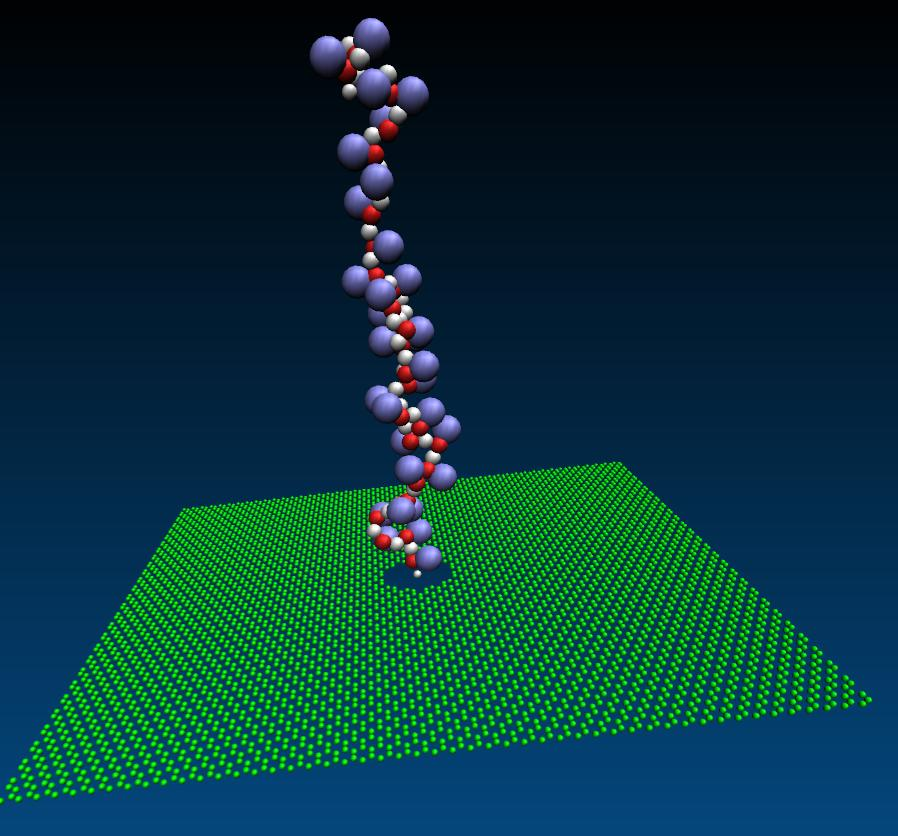
\includegraphics[width=0.6\textwidth]{systemmodlo.jpg}
\caption{Polymère avant la translocation. Les grains de la membrane sont en vert, le squelette du polymère en rouge et blanc. Les grains latéraux violets sont liés aux grains rouges du squelette.}
\label{sytmod}
\end{center}
\end{figure}

\subsubsection*{Les équations du mouvement:}

Nous avons aussi pris en compte des interactions dont nous n'avons pas encore discuté, celles avec le solvant. Il est naturellement hors de question de représenter des molécules de solvant et de calculer leur trajectoire. Nous modéliserons la contribution du solvant de deux façons, une partie de Stokes drag qui représente le frottement et une partie de bruit thermique. De plus, les dimensions nanométriques du systèmes impliquent un nombre de Reynolds\footnote{Le nombre de Reynolds est le rapport des échelles de temps caractéristiques inertielles et visqueuses} très faible. On va donc négliger les termes inertiels des équations de Newton.

Nous obtenons donc pour les équations du mouvement appliquées à chacun des grains composants notre système, l'équation dite de Langevin:
\begin{eqnarray}
\large{
\frac{d \textbf{r}_n}{dt} = - \frac{1}{\nu_n}\frac{\partial U_{n}}{\partial \textbf{r}_n}   + \textbf{g}_n}
\label{langevin}
\end{eqnarray}



Avec $\textbf{r}_n$ la position du grain $n$, $t$ le temps, $U_{n}$ la somme des différents potentiels appliqués au grain $n$, $\nu_n$ le coefficient de frottement de $n$ et $\textbf{g}_n$ la contribution brownienne au mouvement. Cette contribution brownienne présente les propriétés suivantes: sa moyenne est nulle, sa variance est proportionnelle à la température. C'est à dire:
\begin{eqnarray}
\left<\textbf{g}_n\right>\text{}=\text{} 0\text{ , } \left<\textbf{g}_n^2\right>\text{}=\text{} 2 k_B T
\end{eqnarray}

Pour l'ensemble des grains de notre système nous avons choisi, arbitrairement pour la membrane, et comme l'on fait Margaret C Linak et collaborateurs \cite{jchem} pour le polymère de fixer la valeur de $\nu$ à 1 (unité de Lennard-Jones). La valeur de $k_B T$ est estimée en unité d'$\epsilon$ et a été estimée à $1.5$ $\epsilon$ afin de reproduire les conditions expérimentales à température ambiante \cite{jchem}. Notons que nous avons choisi de ne pas prendre en compte les interaction hydrodynamiques entre grains via le solvant.\\

Un fichier caractérisant le système ainsi qu'une liste d'instructions sont fournis à un solveur de dynamique moléculaire, LAMMPS \cite{lammps}, afin de réaliser nos simulations.




\newpage
\section{Modèles théoriques et résultats numériques}

\subsection{Polymères idéaux et non idéaux}
Nous allons dans un premier temps présenter un modèle naïf de polymère idéal afin de poser les bases admises en physique des polymères \cite{sung,these}.\\

Le polymère évolue sur un réseau périodique de paramètre $\lambda$. La tête du polymère est placée sur un des nœuds du réseau. Les monomères consécutifs sont placés sur un des $z$ ($z=4$ pour un réseau carré) sites plus proches voisins, le polymère réalise alors une marche aléatoire (Figure \ref{resideal}).

\begin{figure}[H]
\begin{center}
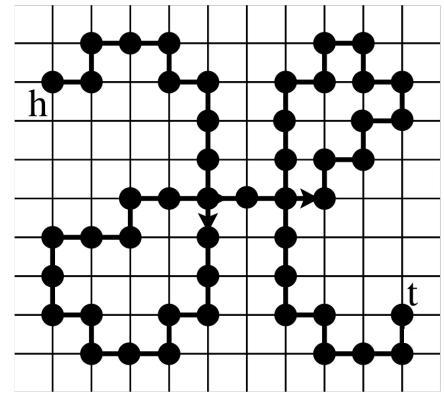
\includegraphics[width=0.25\textwidth]{resideal.jpg}

\caption{Réseau carré montrant la marche aléatoire qui génère une configuration d'un polymère \cite{these}.}
\label{resideal}
\end{center}
\end{figure}

On déduit facilement que pour un degré de polymérisation $N+1$, il y a $Z_{ideal}=z^N$ polymères distincts possibles. Recalculons les résultats fondamentaux concernant la marche aléatoire génératrice du polymère (ces résultats sont indépendants du réseau qui est un artifice de calcul et ne modifie pas les lois d'échelle, pour rappel, la dynamique moléculaire n'utilise pas de maillage). Soit $\textbf{r}$ le vecteur position du marcheur par rapport à l'origine et $b$ la taille d'un pas effectué par le marcheur. Soit $\textbf{r}_n$ le $n$-ième pas effectué, au bout d'un nombre de pas $N$, on a: 

\begin{eqnarray}
\textbf{r} = \sum_{n = 1}^{N} \textbf{r}_n
\end{eqnarray}

Pour la marche aléatoire idéale, il n'y a pas de corrélation entre les différents pas, ce qui mathématiquement se traduit par $\left<\textbf{r}_i \cdot \textbf{r}_j\right> = \delta_{i,j} b^2$. Ce qui implique les relations suivantes:

\begin{eqnarray}
\left<\textbf{r}\right>\text{} = \sum_{n = 1}^{N} \left<\textbf{r}_n \right>\text{} =\text{} 0 \text{ }, \text{} \left<\textbf{r}^2\right> \text{}= \sum_{i = 1}^{N} \sum_{j = 1}^{N} \left<\textbf{r}_i \cdot \textbf{r}_j\right> \text{}= \sum_{i = 1}^{N} \left<\textbf{r}_i^2\right> \text{}= b^2 N
\label{rdmwalk}
\end{eqnarray}

 Puisque la valeur moyenne de $\textbf{r}$ est nulle, on estime le comportement de la distance entre les extrémités (distance end-to-end) moyenne du polymère en prenant la racine carré de la valeur moyenne de $\textbf{r}^2$. Comme le montre l'équation \ref{rdmwalk} la distance end-to-end du polymère sera proportionnelle à $N^\frac{1}{2}$.\\
 
 Une estimation correcte de la taille du polymère est obtenue en considérant le rayon de giration $R_g$. Il est défini de la manière suivante en notant $\textbf{r}_{CM}$ la position du centre de masse du polymère :
 \begin{eqnarray}
R_g^2\text{}=\text{}\frac{1}{N}\sum_{n = 1}^{N} \left<(\textbf{r}_n-\textbf{r}_{CM})^2\right>
 \text{ ou encore, de manière équivalente: }
R_g^2\text{}=\text{}\frac{1}{2N^2}\sum_{i,j}^N \left<(\textbf{r}_i-\textbf{r}_{j})^2\right>
\label{equ}
\end{eqnarray}
 
 L'équivalence s'obtient en développant les termes des deux expressions et en les identifiant.\\


On va appliquer la dernière partie de l'équation \ref{rdmwalk} pour la marche aléatoire à l'équation \ref{equ} du rayon de giration en notant le fait qu'on effectue une marche aléatoire de $|i-j|$ pas pour aller du monomère $i$ au $j$ dans l'expression $\left<(\textbf{r}_i - \textbf{r}_j)^2\right>$.

\begin{eqnarray}
R_g^2\text{}=\text{}\frac{1}{2N^2}\sum_{[|i-j|]} |i-j| b^2=\text{}\frac{1}{N^2}\sum_{[i>j]} |i-j| b^2 =\text{}\frac{b^2}{N^2} \sum_{i=1}^N \sum_{j=1}^{i} j = \text{}\frac{b^2}{N^2}[\frac{1}{2}(\frac{N(N+1)(2N+1)}{6}+\frac{N(N+1)}{2})]
\label{gyr}
\end{eqnarray}

En prenant la limite $N \gg 1$ dans l'équation précédente (\ref{gyr}), on obtient la loi d'échelle à laquelle le rayon de giration obéit:
\begin{eqnarray}
R_g^2\text{}\sim\text{}\frac{b^2}{6}N \Rightarrow R_g\propto N^{\frac12}
\end{eqnarray}

La distance end-to-end et le rayon de giration obéissent à la même loi d'échelle et sont caractéristiques de l'expansion spatiale du polymère.\\


Revenons à notre modèle sur réseau afin d'établir une équation différentielle sur la probabilité, $P(\textbf{r},N)$, du $N$-ième monomère d'être en $\textbf{r}$. Pour cela, introduisons les z $\textbf{b}_i$  vecteurs les plus proches de la position $\textbf{r}$ pour obtenir:
\begin{eqnarray}
P(\textbf{r},N)= \frac{1}{z}\sum_{i=1}^{z} \left[P(\textbf{r}-\textbf{b}_i,N-1)\right]
\label{eqdifprob}
\end{eqnarray}

On effectue ensuite un développement limité à l'ordre 2 afin d'obtenir une équation différentielle à résoudre sur la probabilité de distribution. On fait comme hypothèse que $\textbf{r}>>\textbf{b}_i$ et $N >> 1$.

\begin{eqnarray}
P(\textbf{r}-\textbf{b}_i,N-1)=P(\textbf{r},N)- \frac{\partial P}{\partial N}-  \textbf{b}_{i\alpha} \frac{\partial P}{\partial r_{\alpha} } + \frac12 \textbf{b}_{i\alpha}\textbf{b}_{i\beta} \frac{\partial ^2 P}{\partial r_{\alpha}\partial r_{\beta} }
\end{eqnarray}

En utilisant la convention de sommation d'Einstein, $i$ varie de $1$ à $z$ et $\alpha$ et $\beta$ représentent les coordonnées spatiales. En considérant les résultats suivants:

\begin{eqnarray}
\sum_{i=1}^{z}\textbf{b}_{i\alpha}=0 \text{ },\text{ } \sum_{i=1}^{z}\textbf{b}_{i\alpha}\cdot\textbf{b}_{i\beta} = \frac{b^2\delta_{\alpha,\beta}}{3}
\end{eqnarray}

On obtient l'équation différentielle qui régit la probabilité de distribution de nos monomères:
\begin{eqnarray}
 \frac{\partial P}{\partial N} =   \frac{b^2}{6}\frac{\partial ^2 P}{\partial ^2 \textbf{r}}
 \label{eqdif}
\end{eqnarray}

Cette équation différentielle (\ref{eqdif}) a pour solution avec pour condition initiale $\textbf{r}=0$ quand $N=0$ :
\begin{eqnarray}
P(\textbf{r},N)=\left(\frac{3}{2\pi N b^2}\right)^\frac{3}{2}\exp\left(-\frac{3\textbf{r}^2}{2 N b^2}\right)
\end{eqnarray}

La distribution de probabilité de présence des monomères est donc gaussienne, un polymère idéal est d'ailleurs souvent dit gaussien.\\

Remarquons dors et déjà que le logarithme de la distribution de probabilité donne par définition l'énergie libre du système qui n'est pas sans rappeler celle d'un ressort:
\begin{eqnarray}
F(\textbf{r})= - k_B T \ln(P(\textbf{r},N))= F(0)+\frac{3k_BTr^2}{2Nb^2}
\label{elibre}
\end{eqnarray}
$k_B$ est la constante de Boltzmann. Cette énergie sera utilisée par la suite pour décrire des propriétés dynamiques du polymère.\\



Bien entendu ce modèle est simpliste, un vrai polymère ne peut en aucun s'intersecter lui même, les monomères peuvent être différents, il peut ne pas être linéaire...\\

 Traitons le cas d'un polymère qui ne peut s'intersecter lui-même. Les configurations sont alors générées par des marches aléatoires auto-évitantes (Self Avoiding Walks ou SAW). Soit $v_c \propto b^3$ le volume exclusif occupé par un monomère. La probabilité qu'un monomère de la chaîne de volume $R^3$ ne se superpose pas à un autre est $(1-\frac{v_c}{R^3})$, il y a $\frac{N(N-1)}{2}$ paires de monomères. La probabilité totale de non superposition est donc:
 \begin{eqnarray}
P_{ns}(N)= \left(1-\frac{v_c}{R^3}\right)^{\frac{N(N-1)}{2}} = \exp\left[\frac{N(N-1)}{2}\text{ }\ln\left(1-\frac{v_c}{R^3}\right)\right]
\end{eqnarray}

La probabilité de distribution d'une SAW est donc le produit des deux probabilités précédentes, ce qui donne dans la limite $N \gg 1$, $R \gg v_c$:
\begin{eqnarray}
P_{SAW}(R,N)=P_{ns}(N) P(R,N)=\exp\left[-\frac{3R^2}{2 N b^2}-\frac{v_cN^2}{2R^3}\right]
\end{eqnarray}

La taille caractéristique du polymère est alors donnée par la valeur $R^*$ qui maximise la probabilité de distribution, d'où:
\begin{eqnarray}
\frac{\partial P_{SAW}(R,N)}{\partial R}\HUGE{|} _{R=R^*}=0 \text{ }\Rightarrow \frac{3R^{*2}}{Nb^2}-\frac{3v_cN}{2R^{*4}} =0  \text{ }\Rightarrow R^* \propto N^\frac{3}{5}
\end{eqnarray}


La taille caractéristique du polymère croit donc plus rapidement avec le nombre de monomères que dans le cas idéal précédent. L'exposant 3/5 trouvé est très proche de l'exposant de Flory, $\nu=0.588$, qui fait consensus (réf) parmi les différentes simulations numériques. \\

L'équipe dans laquelle j'ai travaillé avait déjà étudié le comportement d'un polymère linéaire présentant les mêmes caractéristiques que celui du modèle que j'ai développé, hormis la présence de grains le long du squelette du polymère.
La loi d'échelle trouvée pour le rayon de giration est $R_g^2 \propto N^{1.23}$ (courbe disponible en annexe). Cette valeur est légèrement supérieure à la valeur $2\nu=1.176$ attendue. Cette différence peut avoir deux origines: Le volume exclu mal défini par le potentiel de Lennard-Jones qui n'est pas aussi abrupte qu'un échelon infini pour une sphère dure, ainsi que la distance entre les monomères liés qui est sujette à une distribution et n'est pas fixée.\\

En ce qui concerne notre modèle, nous nous attendons aussi à une valeur plus élevée. En effet les même sources d'augmentation sont présentes. De plus, la présence d'un grain latéral sur le squelette linéaire va augmenter la rigidité de notre polymère. Cette rigidité supplémentaire va augmenter les effets de taille fini. Le squelette sera alors plus longiligne, ce qui aura pour effet d'augmenter plus fortement sa taille effective lorsque $N$ croît. Nous avons décidé de tester cette hypothèse.\\

Afin de connaitre l'évolution de la taille de notre système avec le nombre de monomères nous avons laissé évoluer librement notre polymère pendant un nombre important de pas de dynamique moléculaire (jusqu'au milliard pour les chaînes les plus longues). Cela génère un nombre important de configurations du polymère à l'équilibre. Toutefois, ces configurations ne sont pas indépendantes les unes des autres.\\

Pour connaitre l'indépendance de nos configurations, nous avons défini une fonction d'auto-corrélation, $G(H,\tau)$ qui dépend d'une observable $H$ et du temps $\tau$ écoulé entre deux mesures de cette observable.
\begin{eqnarray}
G(H,\tau)=\frac{\left<H(t+\tau)H(t)\right> -\left<H(t)\right>^2}{\left<H(t)^2\right> -\left<H(t)\right> ^2}
\end{eqnarray}

Un scripte en langage C a été utilisé afin de calculer la fonction d'auto-corrélation pour le rayon de giration et la distance end-to-end à partir des données brutes générées par Lammps. Dans un premier temps la moyenne et la variance de l'observable sont calculées. Ensuite, un balayage avec une fenêtre de largeur glissante est effectué avec plusieurs valeurs de $\tau$ afin de calculer la quantité $\left<H(t+\tau)H(t)\right>$. Ci dessous, la Figure \ref{correlgyr} présente $G(R_g,\tau)$ pour différentes tailles de chaîne. L'auto-corrélation de la distance end-to-end est présentée en annexe.


\begin{figure}[H]
\begin{center}
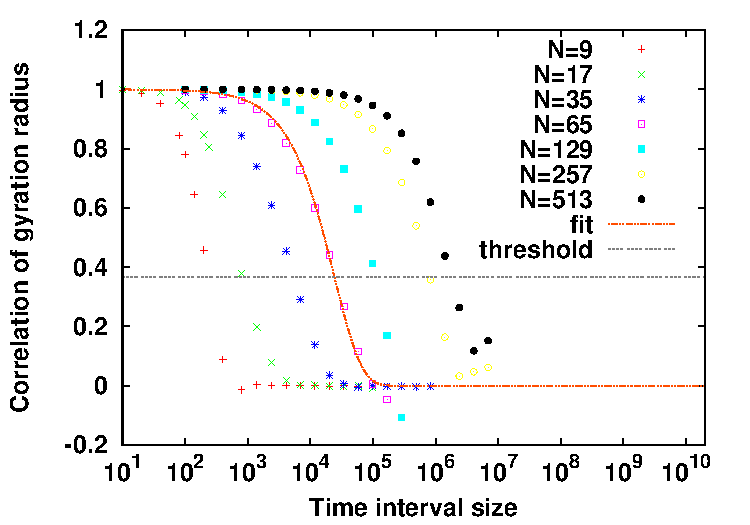
\includegraphics[width=0.55\textwidth]{correlgyr.pdf}
%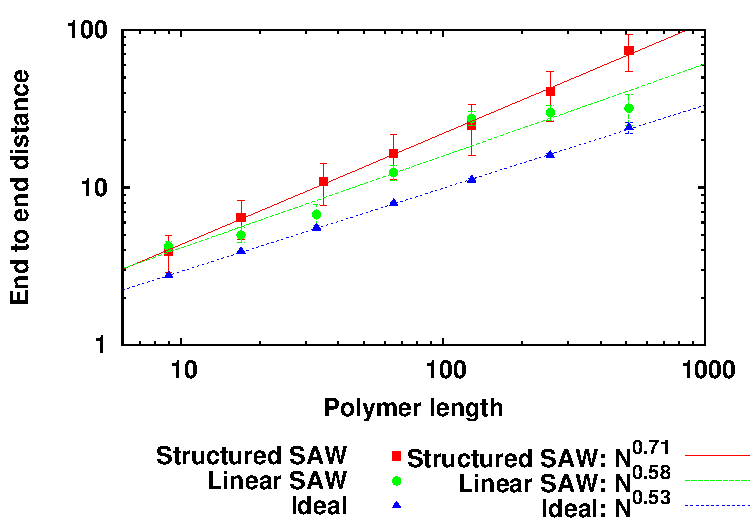
\includegraphics[width=0.49\textwidth]{endtoenddistance.pdf}
\caption{Auto-corrélation du rayon de giration en fonction du temps ($5\cdot10^{-3}$ unité de Lennard-Jones). Les temps de corrélations, déduits avec un fit exponentiel, sont utilisés pour établir le nombre de mesures indépendantes afin d'estimer les barres d'erreurs.}
\label{correlgyr}
\end{center}
\end{figure}

La valeur du temps $\tau(N)$ associé au fit exponentiel $(\exp(-t/\tau))$ est utilisée pour estimer l'erreur sur la moyenne de $R_g(N)$ (explications disponibles en annexe). Nous discuterons de l'évolution de $\tau(N)$ dans le paragraphe suivant. Une loi de puissance est testée afin d'estimer la loi d'échelle suivie par le rayon de giration de notre modèle de polymère. Nous obtenons $R_g \propto N^{0.68}$, ce qui est comme nous nous y attendions supérieur à la valeur trouvée pour un polymère linéaire. Ces données sont présentées dans la Figure \ref{gyr}. Pour la distance entre les extrémités de la chaîne, nous obtenons également un exposant plus élevé $(\nu=0.688)$ que pour le modèle linéaire. Curieusement les deux exposants trouvés différent légèrement. La présence des grains latéraux pourrait contraindre la chaîne à un comportement plus linéaire, d'où une augmentation de l'exposant pour la distance aux extrémités. Les effets de tailles finies sont plus importants pour la distance entre les extrémités.

\begin{figure}[H]
\begin{center}
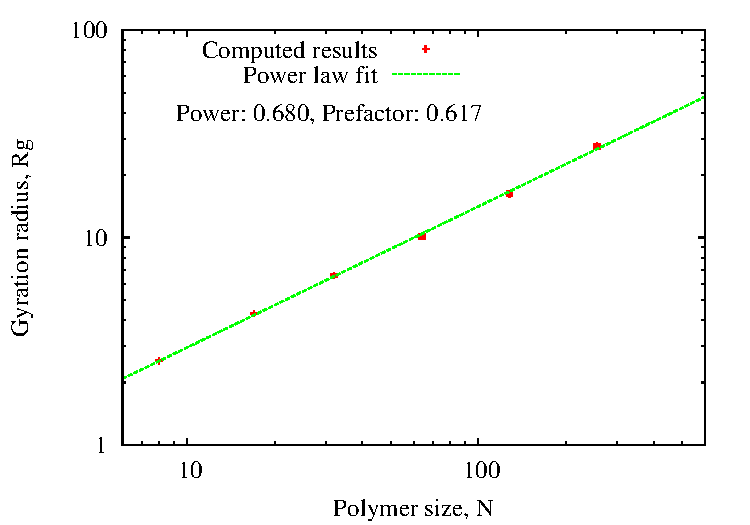
\includegraphics[width=0.55\textwidth]{gyrationradius.pdf}
%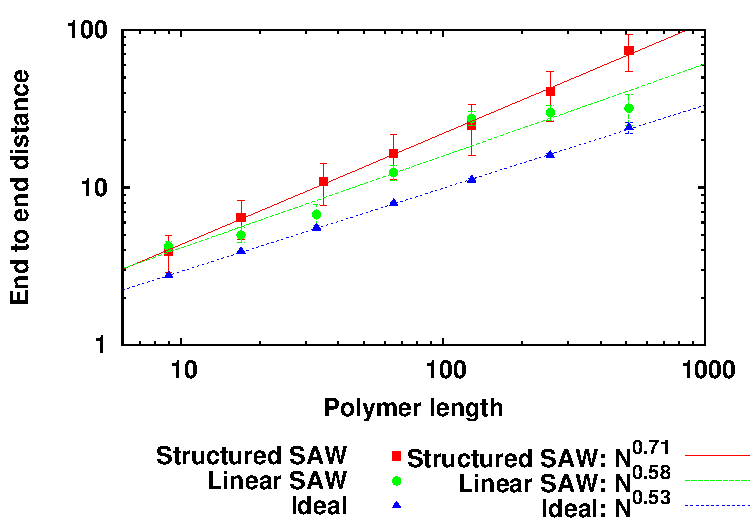
\includegraphics[width=0.49\textwidth]{endtoenddistance.pdf}
\caption{Evolution du rayon de gyration avec le nombre de monomères. Le rayon de giration et la distance end-to-end suivent des lois d'échelle avec des exposants plus élevés que pour un polymère linéaire. $R_g \propto N^{0.680}$ et $|\textbf{r}_N| \propto N^{0.688}$ (graphe pour la distance end-to-end disponible en annexe) }
\label{gyr}
\end{center}
\end{figure}




\subsection{Dynamique des polymères}

Nous allons maintenant proposer un modèle permettant d'aborder la dynamique d'une chaîne. Il s'agit du modèle de Rouse (Figure \ref{rouse}). Comme nous l'avions signalé, l'énergie libre d'un polymère idéal présente les caractéristiques d'un potentiel harmonique de type ressort (cf: équation \ref{elibre}), ce qui justifie cette modélisation.

\begin{figure}[H]
\begin{center}
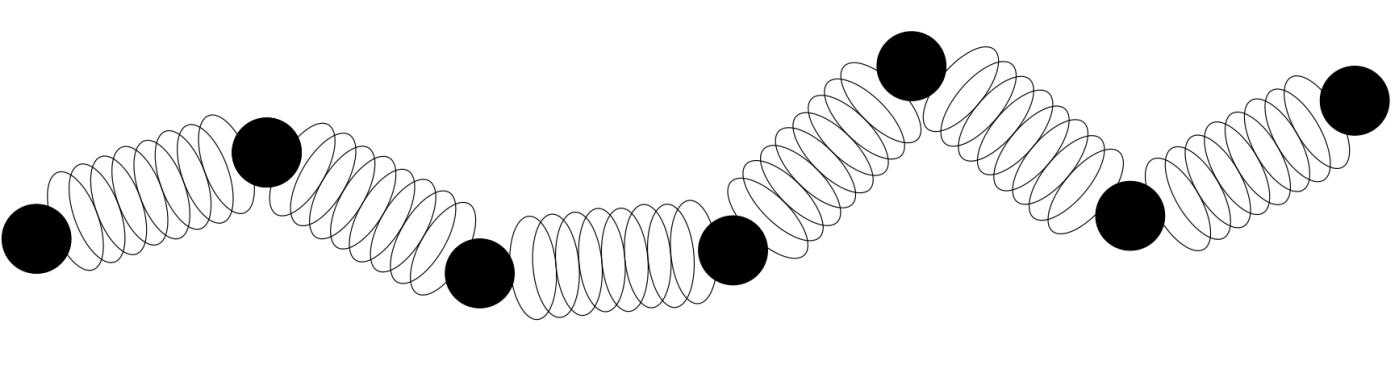
\includegraphics[width=0.45\textwidth]{rouse.jpg}

\caption{Modélisation du polymère par une chaîne d'oscillateurs.}
\label{rouse}
\end{center}
\end{figure}

Le polymère est modélisé par une chaîne d'oscillateurs (de type billes/ressorts). Physiquement, le ressort ne représente pas une liaison entre monomères mais plutôt une partie du polymère assez longue pour que la statistique gaussienne puisse lui être appliquée. De l'équation \ref{elibre} obtenue précédemment on déduit l'énergie élastique du ressort connectant les billes $n$ et $n+1$ séparées par une distance d'équilibre moyenne $b$:


\begin{eqnarray}
F_{n,n+1} = \frac{3 k_B T}{2} \frac{(\textbf{r}_{n+1}-\textbf{r}_n)^2}{b^2}
\end{eqnarray}

Nous nous plaçons dans les conditions décrites lors de l'élaboration du modèle, la trajectoire est donc donnée par l'équation de Langevin \ref{langevin} qui s'écrit ici:

\begin{eqnarray}
\large{
\frac{d \textbf{r}_n}{dt} =  \frac{3T}{\nu_n b^2}( \textbf{r}_{n+1} +\textbf{r}_{n-1} -2\textbf{r}_n )  + \textbf{g}_n}
\end{eqnarray}

On va résoudre cette équation prenant $n$ comme variable continue.

\begin{eqnarray}
\large{
\frac{d \textbf{r}}{dt} =  \frac{3T}{\nu b^2}\frac{\partial ^2 \textbf{r}}{\partial  n^2} + \textbf{g}_n}
\end{eqnarray}

Avec les conditions limites $\frac{\partial  \textbf{r}}{\partial  n}=0$ en bouts de chaine, on peut résoudre le système en le séparant en plusieurs modes à  partir de coordonnées normalisées: 
\begin{eqnarray}
\textbf{x}_p= \frac{1}{N} \int_0^N \cos \left(\frac{n\pi p}{N}\right) \text{ }\textbf{r}(n,t)\text{ } dn \text{ , } \frac{d \textbf{x}_p}{dt} =  -\frac{k_p}{\nu _p} \textbf{x}_p + \textbf{g}_p
\end{eqnarray}



\begin{eqnarray}
\nu_0=  N \nu \text{ , } \nu_p= 2 N \nu  \text{ , }  k_p=\frac{6T\pi^2 p^2}{N b^2}  \text{ , }  \left<\textbf{g}_{p\alpha}(t) \cdot \textbf{g}_{q\beta}(t')\right> = 2\delta_{p,q} \delta_{\alpha ,\beta} \frac{T}{\nu_p} \delta(t-t')
\end{eqnarray}

En travaillant dans la nouvelle base orthogonale, on peut montrer que:


\begin{eqnarray}
\left<(\textbf{x}_{0}(t)-\textbf{x}_{0}(0))_\alpha \cdot (\textbf{x}_{0}(t)-\textbf{x}_{0}(0))_\beta \right> = 2 \delta_{\alpha ,\beta} \frac{T}{N\nu}t
\end{eqnarray}

\begin{eqnarray}
\left<\textbf{x}_{p\alpha}(t) \cdot \textbf{x}_{q\beta}(0)\right> = 2\delta_{p,q} \delta_{\alpha ,\beta} \frac{T}{k_p} \exp\left(-\frac{t}{\tau_p}\right) \text{ , } \tau _p = \frac{\nu N^2 b^2}{3\pi^2p^2T}
\end{eqnarray}

La distance end-to-end et le rayon de giration sont de combinaisons linéaires des $\textbf{x}_p$ et sont donc assujettis  au temps de relaxation le plus long, $\tau_1$ qui obéit à la loi d'échelle : $\tau_1 \propto N^2$. De même la position du centre de masse est donnée par $\textbf{x}_0$, ce qui permet d'en déduire le coefficient de diffusion du polymère:


\begin{eqnarray}
\left<(\textbf{r}_{CM}(t)-\textbf{r}_{CM}(0))^2\right>=\frac{6 k_B T}{N \nu} t = 6 D_R t
\label{fluctudissip}
\end{eqnarray}

L'équation précédente (\ref{fluctudissip}) traduit le théorème de fluctuation dissipation  en prenant en compte $N \nu$, le coefficient de Stokes global du polymère. Le temps de relaxation peut également être vu comme le temps mis par le centre de masse pour parcourir sa longueur. On a alors $\tau \propto \frac{R_0^2}{D}$, soit $\tau \propto N^2 $ dans le cas idéal ou $\tau \propto N^{1+2\nu} $ dans le cas de la marche auto-évitante, ce qui n'est pas observé expérimentalement à cause des interactions hydrodynamiques.\\

Lorsque nous avons défini la fonction d'auto-corrélation, afin de connaître le nombre de mesures indépendan\- tes pour la distance end-to-end et le rayon de giration (voir Figure \ref{correlgyr}), nous avons également vérifié la dépendance en $N$ des temps de corrélation. Nos simulations numériques donnent pour notre polymère, un comportement d'échelle proche de celui d'un polymère auto-évitant. Nous trouvons $\tau_{gir} \propto N^{2.194}$ et $\tau_{e-e} \propto N^{2.132}$. Ces exposants sont plus faibles que le $1+2\nu$ que nous attendions avec la valeur de $\nu$ plus élevée que nous avons trouvé précédemment. Cependant ces valeurs sont compatibles avec la valeur de $\nu$ trouvée dans le cas du polymère linéaire. En effet, le temps de relaxation est lié aux nombre de monomères et à la nature de la liaison ayant la plus faible fréquence (le temps le plus long pilote la relaxation). Ainsi l'agencement stérique du polymère influe sur sa façon d'occuper l'espace, mais pas sur sa dynamique d'équilibre.\\

En ce qui concerne la diffusion du centre de masse, nous avons également vérifié la pertinence de notre modèle. Nous avons tracté notre polymère par une extrémité à laquelle une force d'amplitude variable était imposée. La mesure de la vitesse permet d'estimer le coefficient de friction. Puis lors d'une évolution libre, nous avons estimé la valeur du coefficient de diffusion du centre de masse. Les résultats sont présentés dans la Figure \ref{fluctu-dissip} (Une étude intéressante, mais non pertinente pour la problématique de ce rapport, a été réalisée sur la distribution de coordonnées du monomère de queue lors de la traction, elle est disponible en annexe).

\begin{figure}[H]
\begin{center}
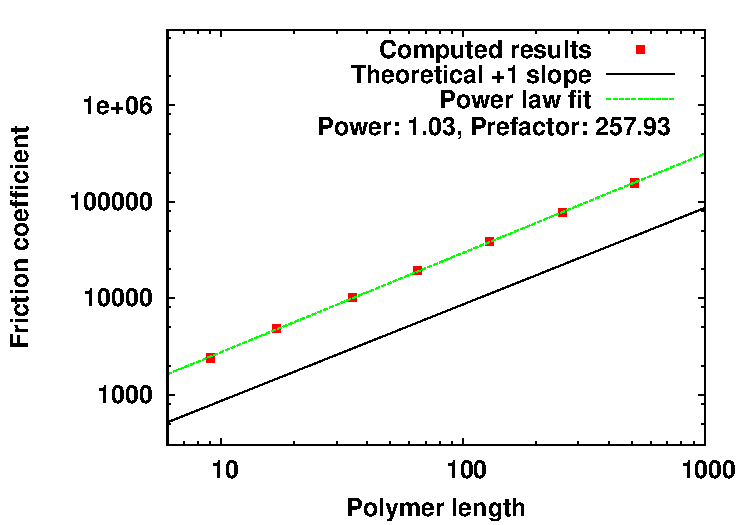
\includegraphics[width=0.5\textwidth]{penteforce.pdf}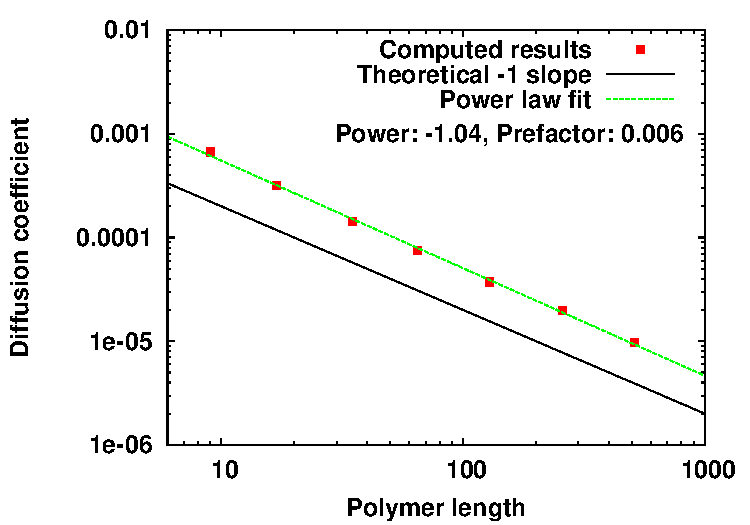
\includegraphics[width=0.5\textwidth]{diffusioncoefficient.pdf}

\caption{A gauche: Evolution linéaire du coefficient de friction total avec la taille du polymère. A droite: Décroissance inverse du coefficient de diffusion avec la taille du polymère. Le produit des pré-facteurs donne une bonne estimation de la température du système. Le théorème de fluctuation-dissipation est vérifié. }
\label{fluctu-dissip}
\end{center}
\end{figure}

On s'attendait a observer une croissance linéaire du coefficient de frottement avec le nombre de monomères, et c'est ce que nous avons trouvé. En effet, le frottement est un effort externe caractérisé par un coefficient de friction local pour chaque grains. La vitesse du centre de masse reflète les efforts externe au système avec pour coefficient de frottement total la somme des coefficients des grains, d'où l'évolution linéaire. Pour le coefficient de diffusion, nous nous attendions également à obtenir $D \propto N^{-1}$ car il est intrinsèquement lié à la friction par le théorème de fluctuation-dissipation. D'ailleurs, le produit des pré-facteurs donne 1.54, ce qui est très proche des 1.5 imposés pour $k_BT$ ( l'étude des données brutes donne 1.497 en moyenne sur toutes les trajectoires pour la température trouvée à l'aide du théorème de fluctuation-dissipation, ce qui est très bon).




\subsection{Translocation}



La translocation peut se dérouler dans différents contextes. Elle peut être due uniquement aux fluctuations thermiques, on parle alors de translocation non biaisée, ou être pilotée par une force extérieure, on parle alors de translocation forcée (driven translocation). Les forces extérieures peuvent être de natures variées, on citera notamment l'utilisation de champs électriques (électrophorèse), de gradients de potentiels chimiques, de flux imposé sur le solvant, ou encore l'emploi de pinces optiques \cite{keyser}.\\

Le temps de translocation dépend alors fortement de la taille du polymère et de la force appliquée, d'une façon générale on peut définir des lois d'échelles:

\begin{eqnarray}
\tau = N^\alpha f^{-\delta}
\label{tau}
\end{eqnarray}

 Le but du stage est de déterminer les valeurs de $\alpha$ et $\delta$, appelés exposants critiques, dans les différentes limites possibles. On basera l'échelle de force en unités de Lennard-Jones à partir de la valeur de $\frac{\epsilon}{b}$.\\

Nous allons dans un premier temps calculer la forme de la barrière d'énergie franchie par le polymère lors de la translocation. Pour cela, nous devons dans un premier temps calculer la probabilité de distribution d'un polymère idéal greffé à une paroi. La chaîne idéale présente comme conditions aux limites, la non pénétration des monomères à travers la paroi. On note $P(\textbf{r},\textbf{r}_0,n)$ la probabilité de trouver le $n$-ième monomère en position $\textbf{r}$, pour $n \gg 1$, le premier monomère étant greffé en $\textbf{r}_0$. $P_0$ est la distribution calculé précédemment pour un polymère idéal libre.

\begin{eqnarray}
P_0(\textbf{r},\textbf{r}_0,n)=\left(\frac{3}{2\pi n b^2}\right)^\frac{3}{2}\exp\left(-\frac{3(\textbf{r}-\textbf{r}_0)^2}{2 n b^2}\right)
\end{eqnarray}

A l'instar de nombreux problèmes d'électromagnétisme ou de mécanique des fluides, on utilise la méthode des images miroirs afin de déterminer $P(\textbf{r},\textbf{r}_0,n)$. En effet, on a:

\begin{eqnarray}
P(\textbf{r},\textbf{r}_0,n) \propto P_0(\textbf{r},\textbf{r}_0,n)-P_0(\textbf{r},-\textbf{r}_0,n)
\end{eqnarray}

Dans le cas idéal, la probabilité de distribution du monomère de queue est à variables séparables. En posant $\textbf{r}_0= \epsilon y$ avec $\epsilon \ll 1$, un développement limité au premier ordre donne:

\begin{eqnarray}
P(\textbf{r},\textbf{r}_0,n) \propto \left(\frac{3}{2\pi n b^2}\right)^\frac{3}{2} \left(\frac{6 y \epsilon}{n b^2}\right)\exp\left(-\frac{3\textbf{r}^2}{2 n b^2}\right)
\end{eqnarray}

Pour le cas non idéal, les termes supplémentaires introduits dans $P_0$ ne permettent pas de séparer les variables et d'obtenir une expression analytique.


\begin{figure}[H]
\begin{minipage}{0.45\linewidth}
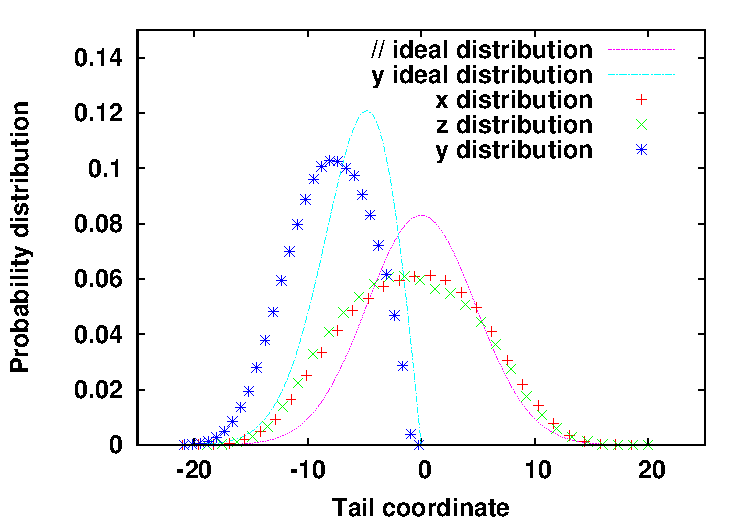
\includegraphics[width=1.2\textwidth]{probdistribution.pdf}

\end{minipage}\hfill
\begin{minipage}{0.45\linewidth}
\caption{Probabilité de distribution théorique du monomère de queue pour un polymère idéal et résultats numériques pour un polymère à monomères durs (N=35). Parallèlement à la membrane, la distribution gaussienne idéale est aplatie au centre à cause de la zone d'exclusion des autres monomères. De même pour la direction perpendiculaire, le pic maximum est repoussé par la présence d'autres monomères. Dans les deux cas, l'éloignement maximal n'est pas modifié car le cas idéal correspond déjà à des chaînes étirées sans superpositions de monomères. }
\label{polagainstwall}
\end{minipage}
\end{figure}


Afin d'aborder la translocation, nous avons du créer des configurations indépendantes de polymères à l'équilibre, juste avant l'application d'une force. Lors de ce processus de génération, nous avons laisser le polymère évoluer librement en fixant une extrémité au centre du pore. L'étude des coordonnées du grain de queue nous a permis d'évaluer l'influence des volumes exclus, comme le montre la Figure \ref{polagainstwall}.


La probabilité de distribution du polymère accolé à une membrane permet, à partir de la fonction de partition stérique, $Z_S(n)= \int_{y>0} P(\textbf{r},\textbf{r}_0,n) \textbf{dr}$, de calculer l'énergie libre d'origine entropique d'un tel système. Dans la limite $n \gg 1$, le premier terme non nul du développement limité impose la loi d'échelle: $Z_S(n) \propto n^{-1/2}$. Pour un polymère de $N$ monomères en cours de translocation, lors du passage du $n$-ième monomère, on obtient la valeur de l'énergie libre en prenant en compte les effets entropiques de part et d'autre de la membrane:
\begin{eqnarray}
F(N,n)= -k_BT\ln\left(Z_S(n)Z_S(N-n)\right)= \frac{1}{2} k_BT \ln \left(n(N-n)\right) +cste
\end{eqnarray}

Cette barrière d'énergie à franchir au cours de la translocation peut être altérée en appliquant une différence de potentiel, chimique ou électrique, ou encore en appliquant directement une force sur la chaîne. La Figure \ref{energiebarrier} montre cette barrière d'énergie.
\begin{figure}[H]
\begin{center}
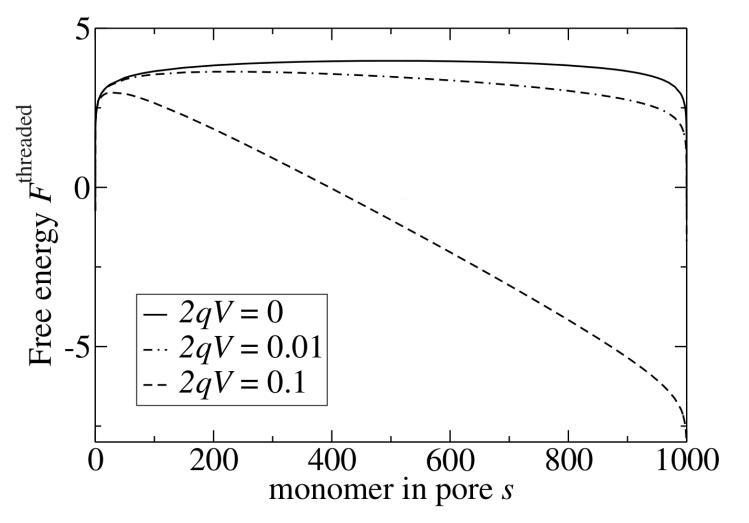
\includegraphics[width=0.4\textwidth]{transelec.jpg} 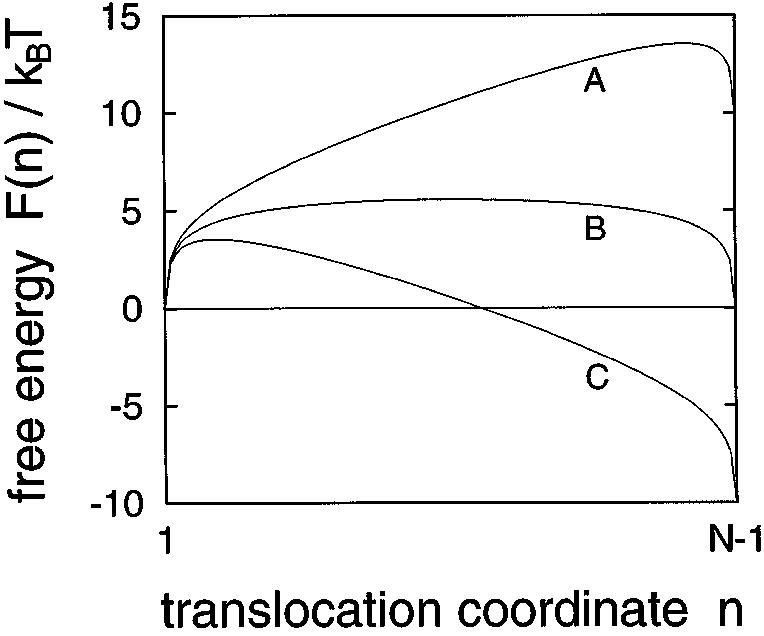
\includegraphics[width=0.28\textwidth]{transpotchim.jpg}

\caption{Modification de la barrière entropique par une différence de potentiel électrique (à gauche \cite{these}) et de potentiel chimique (à droite \cite{sung}). A: différence de potentiel opposée à la translocation, B: différence de potentiel nulle, C: différence de potentiel favorable.}
\label{energiebarrier}
\end{center}
\end{figure}

 Lors de la translocation non biaisée, la barrière d'énergie est utilisée pour résoudre l'équation de Smoluchowski, qui va permettre de déduire $\tau \propto N^{1+2\nu}$ comme limite inférieure. Le cas non biaisé n'a pas été étudié. Le lecteur intéressé trouvera démonstrations et explications dans l'article de revue de Milchev \cite{milchev}.
 
 Pour la translocation forcée, l'application d'une force bouleverse l'hypothèse de l'équilibre thermodynamique local utilisée pour évaluer $\tau$ dans le cas non biaisé. Plusieurs modèles hors équilibre sont présentés dans l'article de J. L. A. Dubbeldam et collaborateurs \cite{traction}. Nous retenons de la lecture de cette article que pour la dépendance en $N$, ils s'attendent à une transition de $\tau \propto N^{2\nu}$ à $\tau \propto N^{1+\nu}$ lorsque la force augmente. En ce qui concerne la dépendance en $F$, ils s'attendent à une transition de $\tau \propto F^{-1}$ à $\tau \propto F^{(1/\nu)-2}$ lorsque la taille de la chaîne diminue.



\subsubsection*{Translocation à travers un pore large}

Dans un premier temps, nous avons considéré une membrane fixe munie d'un nanopore large. Le nanopore est créé en supprimant 54 grains au centre. L'extrémité du polymère est alors tirée par l'ajout d'une force perpendiculaire à la membrane et d'amplitude modulée sur 3 ordres de grandeurs, de 0.1 à 100. Un cylindre de sécurité est implanté dans le code pour vérifier que le pore est toujours peuplé. Lorsque ce n'est plus le cas, nous vérifions si le polymère a terminé sa course du coté cis ou du coté trans. En effet, pour de faibles forces, le polymère peut dans certaines simulations, ne pas effectuer la translocation.\\

Trois polymères ont été étudiés, ils présentent 8, 16 et 32 monomères. A l'instar des prédictions de J. L. A. Dubbeldam et collaborateurs \cite{traction}, nous observons deux régimes distincts caractérisant la dépendance de la loi d'échelle avec la force. En effet, on observe à forces faibles (excepté pour $N=8$) et intermédiaires un comportement tel que $\tau \propto 1/F$. Pour des forces plus élevées, on trouve une loi d'échelle avec un exposant plus élevé ($\tau \propto F^{-0.74}$ pour N=8) Cet exposant plus élevé montre la transition vers $\tau \propto F^{(1/\nu) -2}$. La valeur plus faible qu'attendue peut être attribuée aux effets de taille finie et à l'amplitude de la force qui n'est pas assez élevée. De plus la transition entre les régime semble apparaitre plus tôt pour les $N$ faibles, contrairement à la prédiction de J. L. A. Dubbeldam et collaborateurs \cite{traction}. Cette différence pourrait venir du fait que nous tractons notre polymère (force en bout de chaîne), alors que dans leur cas, une différence de potentiel est appliquée (force au sein du pore). La Figure \ref{holebigger} permet de mieux visualiser ces régimes. En ce qui concerne l'évolution de $\tau$ avec $N$, on trouve un exposant de 1.78 pour les forces imposées de 9 et 20, et 1.69 pour 80. Ces valeurs sont proches du cas $\tau \propto N^{(1+\nu)}$ attendu pour les forces importantes.

Dans le cas $N=8$, nous observons un décrochement de pente. Ceci se produit lorsque la force est faible et pour une chaîne très courte. L'impulsion initiale donnée par le mouvement brownien rejette nombre de configurations (d’où une forte diminution du nombre de translocation réussies), celles conservées ayant une grande impulsion non naturelle dans le sens de la translocation, diminuant artificiellement $\tau$. Cette rupture de pente nous semble donc être un effet de taille finie.

Exercer des forces plus faibles nous ferait perdre beaucoup trop d'événements. Afin de balayer de larges domaines, il pourrait être intéressant de travailler, comme cela peut être fait expérimentalement à vitesse de traction imposée (la force n'est alors plus constante).

\begin{figure}[H]
\begin{center}
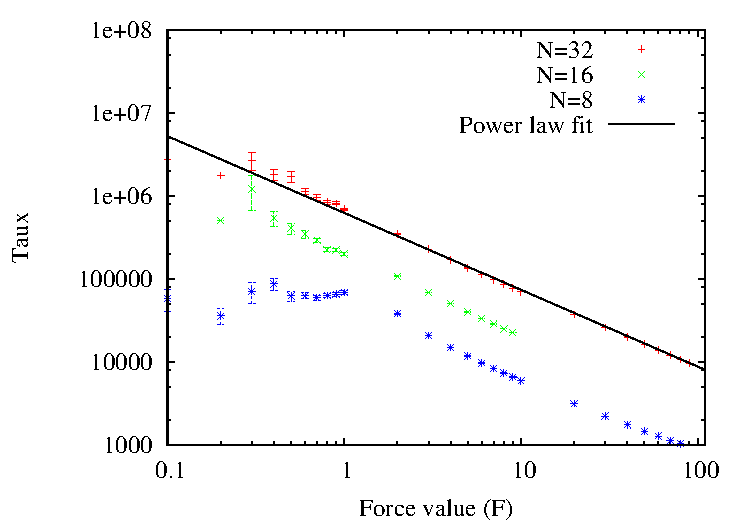
\includegraphics[width=0.48\textwidth]{translocfholebigger.pdf} 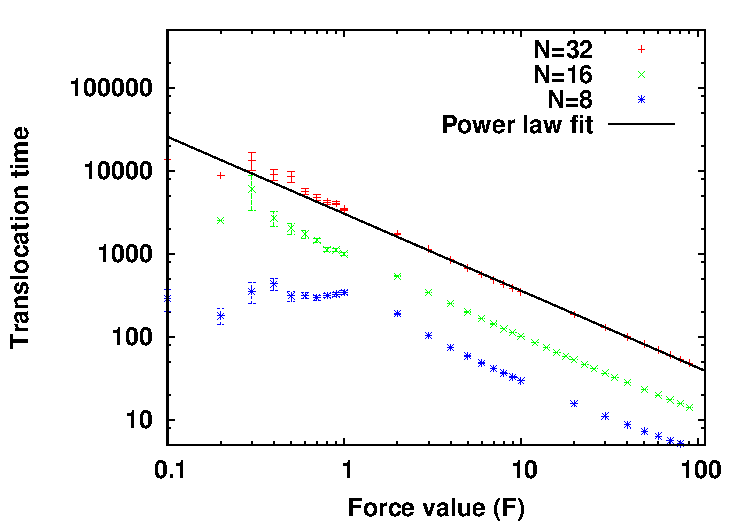
\includegraphics[width=0.48\textwidth]{translocholebigger.pdf}

\caption{Lors de la translocation à travers un pore large, on distingue deux régimes, une décroissance de $\tau \propto 1/F$ suivit d'une augmentation de l'exposant critique quand $F$ devient suffisamment grande. La rupture de pente du cas $N=8$ est imputée à des effets de taille finie. On trouve bien des valeurs proches de $\tau \propto N^{1+\nu}$ pour la dépendance en N.}
\label{holebigger}
\end{center}
\end{figure}

Afin de ralentir la translocation, enjeu clé du séquençage, nous allons maintenant étudier l'influence d'un nanopore plus étroit. En quoi le frottement important induit par le pore va-t-il modifier les lois d'échelle trouvées précédemment?


\subsubsection*{Translocation à travers un pore étroit}
Nous étudions dorénavant l'effet d'une membrane fixe munie d'un nanopore étroit qui va induire un frottement plus important. Le nanopore est créé en supprimant uniquement 24 grains au centre cette fois ci. Le pore a été choisi suffisamment étroit pour empêcher les monomères de passer de front, ils devront se déformer pour permettre le passage du grain latéral, plus volumineux.\\

Encore une fois, nous observons les deux régimes précédents. Cependant la frontière semble apparaitre plus tard à cause du frottement, ce qui diminue la force effective appliquée sur le polymère ($F_{eff}=F-\epsilon _{pore})$. Les mêmes lois d'échelles sont observées à forte force ( $\tau \propto 1/F$ puis $\tau \propto F^{(1/\nu) -2}$).\\

 Une grande différence s'observe dans le cas de l'application de forces faibles. Comme la Figure \ref{thinpore} le suggère, les translocations n'ont pas pu être menées à bien pour des forces inférieures à l'unité.

Les contraintes stériques choisies entrainent une modification de la barrière d'énergie. La translocation des grains par groupe de trois (1 grain latéral volumineux à la fois), comme nous l'illustrerons dans la section suivante (Figure \ref{temperature}), corrobore une hypothèse de déformation de la barrière entropique en dents de scies décroissante. Cette modification est significative puisqu'elle empêche complétement la translocation si la force appliquée est trop faible, elle semble aussi être responsable du comportement inattendu décrit dans la Figure \ref{thinpore}.

Le cas $N=8$ présente encore une fois des problèmes. Lorsque la force est trop faible, les polymères ne pénètrent pas à travers la membrane. Dans le cas de $N=8$, la force est à peine suffisante pour permettre la translocation et n'est pas prépondérente par rapport au bruit thermique. Le polymère passe alors un temps important à rebondir sur le pore avant d'entamer la translocation. Le temps de translocation est alors fortement surévalué (un point a été conservé sur la Figure \ref{thinpore}, pour illustrer ce problème).



\begin{figure}[H]
\begin{center}
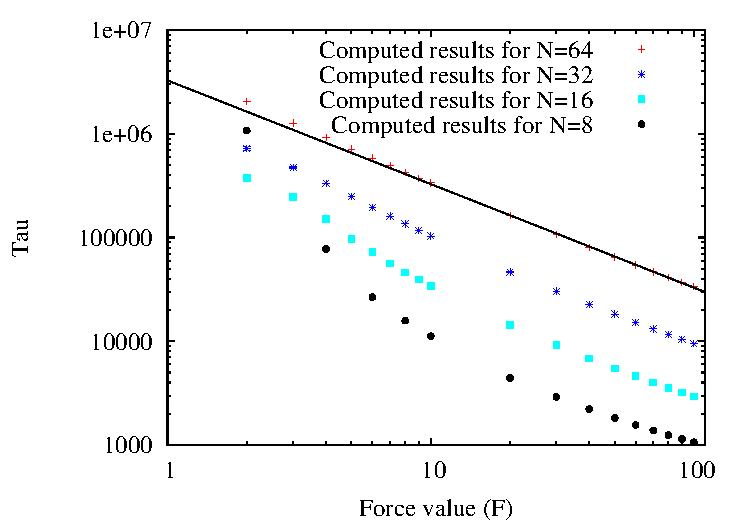
\includegraphics[width=0.48\textwidth]{translocfthinpore.pdf} 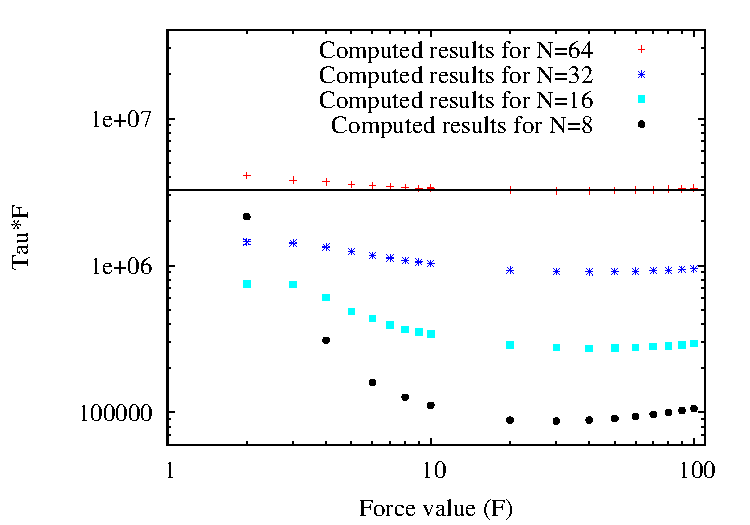
\includegraphics[width=0.48\textwidth]{translocthinpore.pdf}

\caption{Lors de la translocation à travers un nanopore étroit, la transition entre les les deux régimes observés précédemment semble se faire pour des forces plus élevées. Le frottement pourrait être caractérisé par une diminution de la force effective. La loi $\tau \propto N^{1+\nu}$ est toujours suivie. La modification de la barrière d'énergie introduit un comportement imprévu à gauche de la courbe. Le comportement anormal du cas $N=8$ à faible forces est dû a des effets de tailles finies et aux conditions de test lors des simulations.}
\label{thinpore}
\end{center}
\end{figure}

Les lois d'échelles ne semblent pas avoir été modifiées à fortes forces, si ce n'est en introduisant une force effective à cause du frottement. L'application d'une force faible sur un nanopore étroit permet de ralentir la translocation (Figure \ref{both}).

\begin{figure}[H]
\begin{center}
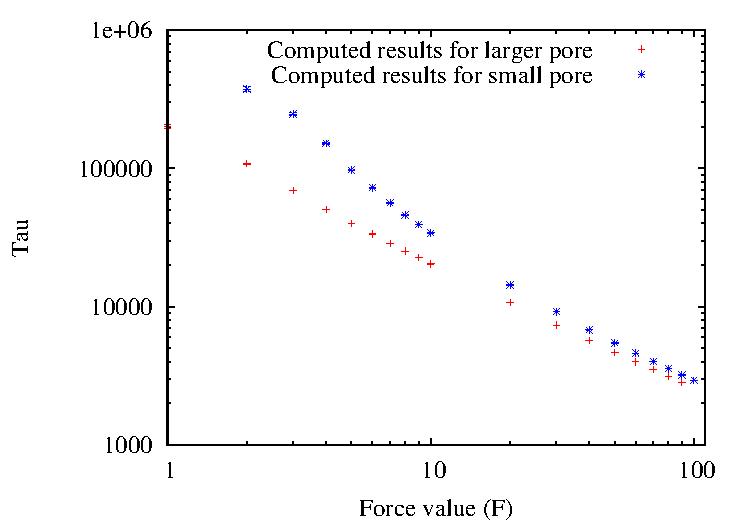
\includegraphics[width=0.45\textwidth]{translocporedifn.pdf} 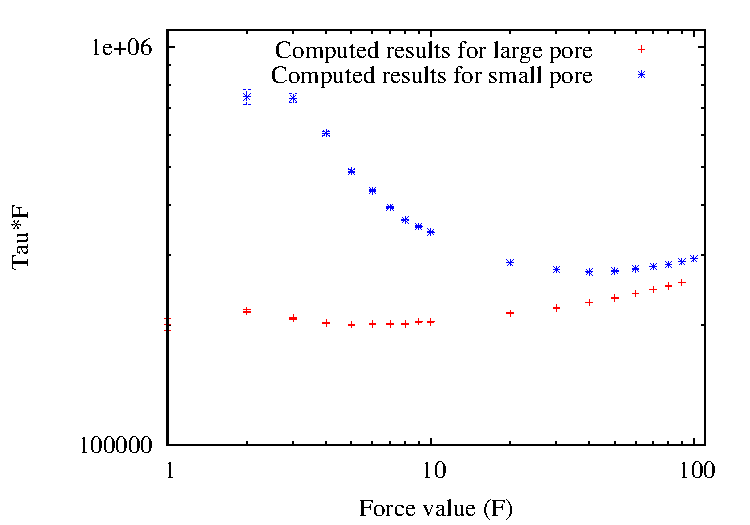
\includegraphics[width=0.45\textwidth]{translocporedif.pdf}

\caption{A forte force, l'étroitesse du pore ne modifie pas les lois d'échelles. A faible force la modification de la barrière énergétique entraine une augmentation importante du temps de translocation (ici $N=16$).}
\label{both}
\end{center}
\end{figure}

Nous allons maintenant nous intéresser à l'influence des propriétés vibrationnelles du graphène sur la translocation.

\subsubsection*{Translocation à travers un pore vibrant}

Pour les vibrations, nous avons choisi de thermaliser notre membrane a une température bien plus faible que celle du polymère ($0.005\epsilon$) afin de pouvoir observé l'échauffement du pore au cours de la translocation. Afin de conserver une trajectoire naturelle, nous avons imposé au potentiel harmonique des carbone une raideur adaptée. La Figure \ref{temperature} commente les résultats observés sur une translocation unique (en ce qui concerne les résultats ayant une signification statistique, nous obtenons des résultats surprenants montrés en annexe).
\begin{figure}[H]
\begin{center}
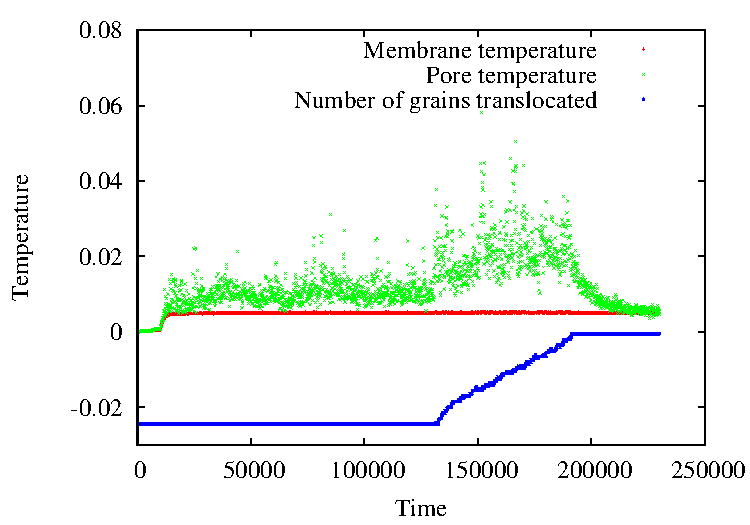
\includegraphics[width=0.49\textwidth]{tempmurmobil.pdf}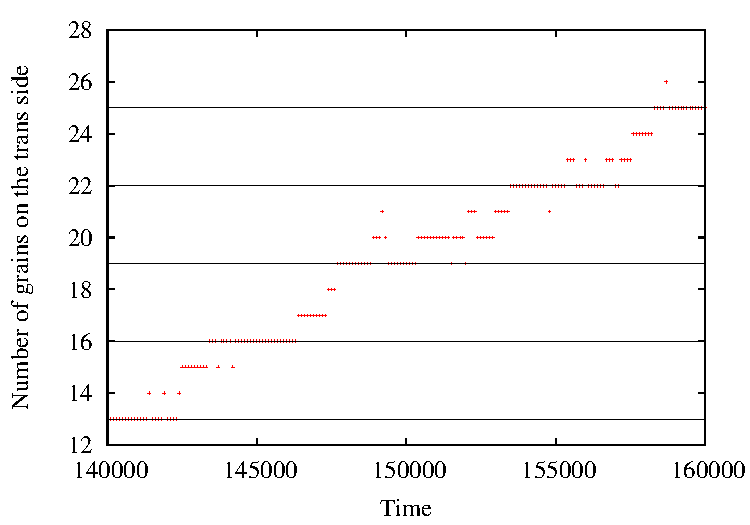
\includegraphics[width=0.49\textwidth]{murmobil.pdf}

\caption{A gauche: Evolution de la température de la membrane et du pore au cours de la thermalisation, suivie de la translocation, le nombre de grains passés du coté trans est donné de manière indicative (échelle arbitraire). Lors de la translocation, le polymère échauffe la paroi du pore, qui retourne à l'équilibre thermique une fois la translocation terminée. A droite: Illustration de la translocation ayant lieu par paliers, le gros grain latéral passant difficilement à travers le pore.}
\label{temperature}
\end{center}
\end{figure}




\section{Conclusion}

Au cours de ce stage, nous avons construit un modèle gros grains de polymère présentant des contraintes stérique comparables à celles de l'ADN. Notre approche est originale, en ce qu'elle consiste à créer un polymère suffisamment détaillé pour reproduire certains comportements de l'ADN, mais suffisamment simple pour vérifier des lois d'échelles prévues par la physique statistique. L'élaboration de ce polymère nous a permis d'évaluer des exposants critiques caractérisant la translocation.\\

Nous avons, dans un premier temps, vérifié la cohérence de notre modèle en retrouvant des résultats connus pour un polymère libre. Ces préliminaires effectués, nous avons trouvé les lois d'échelles régissant notre système, dans le cas d'un nanopore large, ainsi que dans celui, plus original, d'un nanopore étroit modifiant la barrière d'énergie entropique à franchir. Ceci nous a permis de montrer qu'il est possible, à faible forces dans un pore étroit, d'augmenter significativement le temps de translocation, condition préalable à un éventuel séquençage.\\

Ce travail est toujours en cours et sera poursuivie par une thèse dans l'équipe de Arnaud Buhot. Nous nous attacherons donc à mieux comprendre (et corriger si nécessaire) ce qui a été mis en œuvre pour le pore vibrant. En plus de la vibration du pore, nous modéliserons la flexibilité du plan de la membrane dans son ensemble. Enfin, l'utilisation d'une force de type électrique, agissant dans au sein du pore, ou encore un travail à vitesse imposée, pourront être envisagés.




\bibliography{biblio}
\bibliographystyle{ieeetr}

\newpage

\section{Annexe}

\subsection*{Les nanopores}



\subsubsection*{Les bio-pores:}
Les premiers pores étudiés ont été ceux directement disponibles car existants dans la nature, les bio-pores. Le plus utilisé est l'$\alpha$-hémolysine, il s'agit d'une exotoxine produite par le Staphylocoque doré, c'est ce qu'a utilisé l'équipe de Kasianowicz \cite{kasianowicz} en 1996 en réalisant la première translocation d'ADN. Comme l'illustre la Figure \ref{biopore}, l'ADN peut aisément effectuer une translocation à travers une membrane lipidique par le biais de ce pore. \\

\begin{figure}[H]
\begin{center}
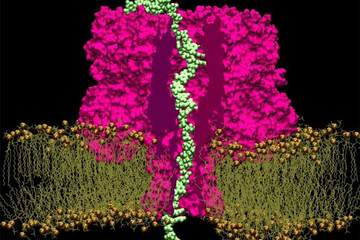
\includegraphics[width=0.45\textwidth]{biopore.jpg}

\caption{Translocation d'ADN grâce à l'$\alpha$-hémolysine, un bio-pore.}
\label{biopore}
\end{center}
\end{figure}

Les bio-pores présentent certains avantages, ils peuvent être cultivés et ont souvent une grande sélectivité vis a vis des molécules autorisées à traverser. Ils permettent ainsi de détecter des protéines ou des ions particuliers. Cependant ils présentent des limitations: leur taille n'est pas modulable, ils nécessitent de travailler en conditions physiologiques. Un des obstacles à leur utilisation pour le séquençage est leur importante épaisseur, comme nous l'avons fait remarquer précédemment.


\subsubsection*{Les pores artificiels classiques:}

Afin de pallier aux désavantages des bio-pores, des pores artificiels ont été élaborés. Ces pores, principalement basés sur les technologies du silicium, perdent en sélectivité, mais ont des propriétés beaucoup plus adaptables, ce qui permet de quantifier l'influence des paramètres géométriques. A l'instar des bio-pores, leur épaisseur reste trop importante. La Figure \ref{artificialpore} présente un exemple de pore en silice.

\begin{figure}[H]
\begin{center}
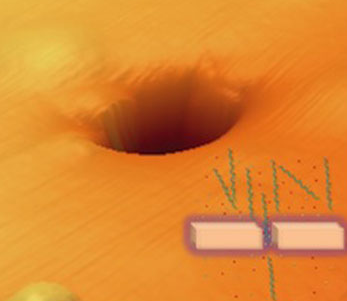
\includegraphics[width=0.3\textwidth]{artificialpore.png} \hspace{0.02\textwidth}
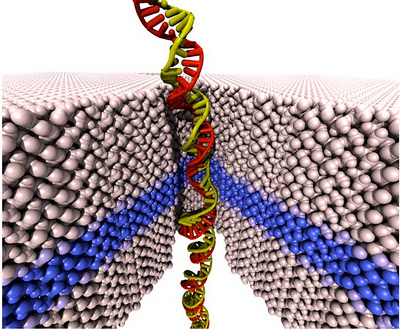
\includegraphics[width=0.35\textwidth]{nanoporeart.jpg}

\caption{Un pore artificiel en silice, imagerie par AFM et modélisation.}
\label{artificialpore}
\end{center}
\end{figure}

Le lecteur intéressé par les possibilités des différents types de pores et l'emploi de divers moyens de contrôles sur la translocation appréciera l'article de revue écrit par Ulrich F. Keyser \cite{keyser}. 

\section*{Unités de Lennard-Jones / Unités S.I}
\begin{center}


\begin{tabular}{|l|c|c|c|}
  \hline
 Système & Dimension & Unités de Lennard-Jones & Unités S.I \\
  \hline
  Etalon de distance & $L$ & $1\cdot\sigma$ & 0.3 nm \\
  Etalon d'énergie & $E$ & $1\cdot\epsilon$ & $1.5\cdot10^{-19}$ J\\
  Force & $E L^{-1}$ & $1\cdot F$ & $5\cdot10^{-10}$ N\\
     
  Echelle de temps & $E^{1/2} M^{-1/2} L^{-1} $ & $1\cdot t$ & $1.3$ s\\
   Coefficient de frottement & $ L^3 E^{-1} T^{-1}$ & $1\cdot \nu$ & $1.4\cdot10^{10}$ m^{3}$\cdot$ J^{-1}$\cdot$ T^{-1}\\
   
  \hline
\end{tabular}
\end{center}

La masse n'apparait pas explicitement dans l'équation de Langevin, elle vaut 1 pour tous les grains et est prise indirectement en compte dans $\nu$. L'échelle de temps, 1.3 secondes semble élevée mais nous travaillons avec des pas de temps $5\cdot 10^{-3}$ fois cette échelle de temps.


\section*{Distance end-to-end}

\begin{figure}[H]
\begin{center}
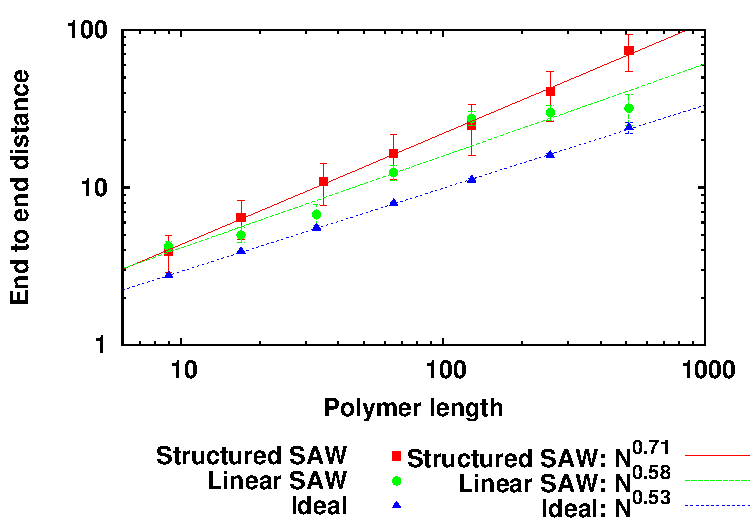
\includegraphics[width=0.55\textwidth]{endtoenddistance.pdf}
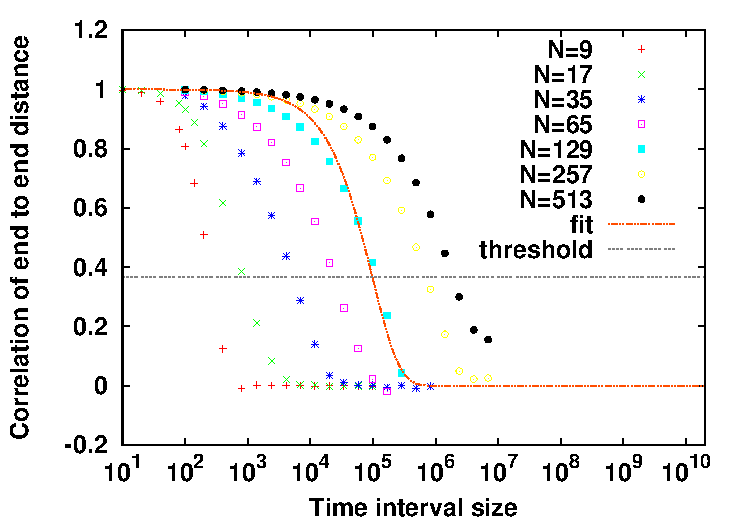
\includegraphics[width=0.55\textwidth]{correlendtoend.pdf}

\caption{Loi d'échelle suivie par la distance entre les extrémités de la chaîne et fonction d’auto-corrélation associée. Le fit exponentiel ne pas marche toujours très bien mais il donne une bonne estimation du temps de corrélation.}
\label{endtoend1}
\end{center}
\end{figure}

\section*{Estimation des barres d'erreurs}

Les temps de corrélation que nous avons estimés pour chaque longueur de chaîne sont mis à contribution pour estimer les barres d'erreurs. Au lieu d'utiliser l'équation \ref{corel},
 comme c'est le cas de manière générale pour $N$ mesures indépendantes d'une observable $A$. Nous avons préféré utilisé une définition différente en considérant que nos mesures sont indépendantes après cinq temps de corrélations, comme le montre l'équation \ref{corel2}.

\begin{eqnarray}
\sigma=\sqrt{\frac{\left<A^2\right>-\left<A\right>^2}{N}}
\label{corel}
\end{eqnarray}

\begin{eqnarray}
\sigma=\sqrt{\frac{\left(\left<A^2 \right>-\left<A \right>^2\right)\left(5 \cdot \tau_c\right)}{N}}
\label{corel2}
\end{eqnarray}

En ce qui concerne le coefficient de diffusion, la méthode est différente, puisqu'il n'est pas mesuré à chaque pas de dynamique moléculaire. La méthode utilisée est décrite dans la Figure \ref{errorbard}.

\begin{figure}[H]
\begin{center}
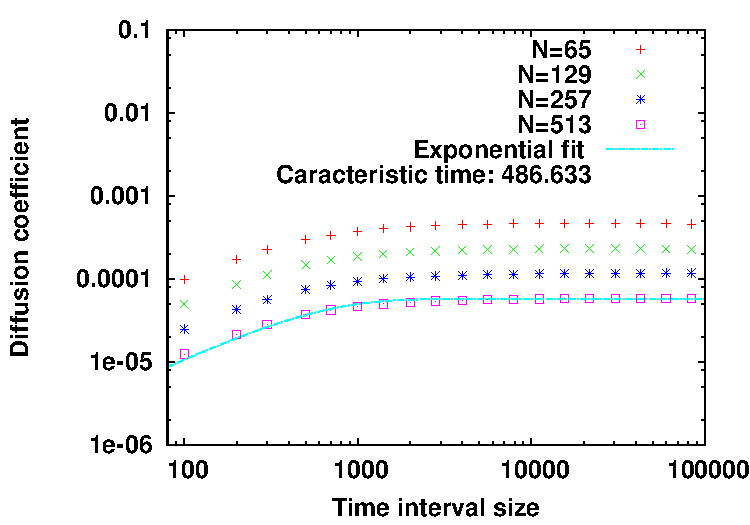
\includegraphics[width=0.8\textwidth]{dexptime.pdf}

\caption{Le coefficient de diffusion est caractéristique de la distance au carrée moyenne parcourue par le centre de masse en un temps $t$ : $\left<x^2\right> =D\cdot t$. Nous avons évalué différentes valeurs de $D$ à l'aide de fenêtres glissantes de tailles $\Delta t$ différentes. Pour les petites fenêtres, la valeur de $D$ est fortement sous évaluée. Nous avons remarqué qu'un fit exponentiel de type $D_0\left(1-\exp\left(-t/\tau\right)\right)$ fonctionne bien et donne quasiment la même valeur de $\tau$ quelque soit le nombre de monomères. $D$ est une caractéristique du centre de masse, il est normal que son amplitude varie avec $N$ car $\nu$ évolue avec $N$, et que $\tau$ reste inchangé car il résulte d’efforts extérieurs. Nous avons choisi une fenêtre de taille $5\cdot \tau$ pour évaluer $\left<D\right> $ et l'équation \ref{corel} pour $\sigma_D$.}
\label{errorbard}
\end{center}
\end{figure}

\newpage

\section*{Traction d'un polymère à fortes forces}

Lorsque nous avons mesuré le coefficient de friction de nos chaînes, nous avons également étudié la distribution des coordonnées du monomère de queue.

\begin{figure}[H]
\begin{center}
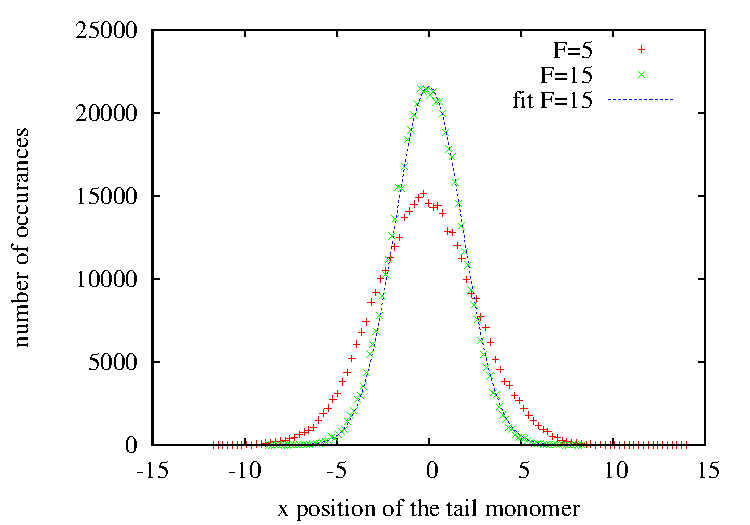
\includegraphics[width=0.5\textwidth]{gausslateral.pdf}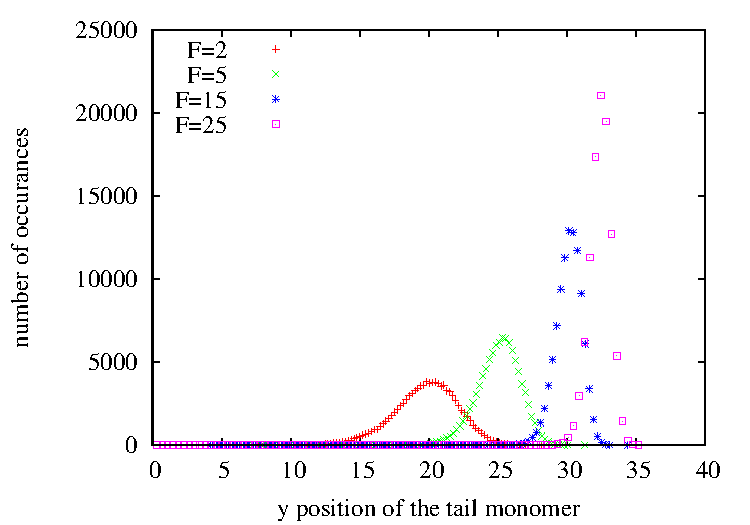
\includegraphics[width=0.5\textwidth]{ydistribtraction.pdf}

\caption{Lorsque la chaîne est tractée à forte force (ici dans la direction y), elle s'étire. On voit comme conséquence de cet étirement que selon la coordonnée x (x queue - x tête),  les effets de volumes exclus de la SAW n'interviennent plus. Les distribution perpendiculaires à la force appliquée retrouvent une distribution gaussienne. Cependant la largeur de cette distribution dépend de la force de traction ; plus on tire fort, plus la queue est rabattue vers le centre. Nous avons évaluer une loi de puissance pour la décroissance de la largeur de la gaussienne à $\sigma \propto F^{-0.3}$, qui reste à comparer avec la littérature. En ce qui concerne la direction y, on constate qu'il existe un pic de probabilité qui est de plus en plus éloigné de la tête et de plus en plus resserré au fur et à mesure que la force augmente. }
\label{traction}
\end{center}
\end{figure}

\section*{Résultats surprenants du pore vibrant}


\begin{figure}[H]
\begin{center}
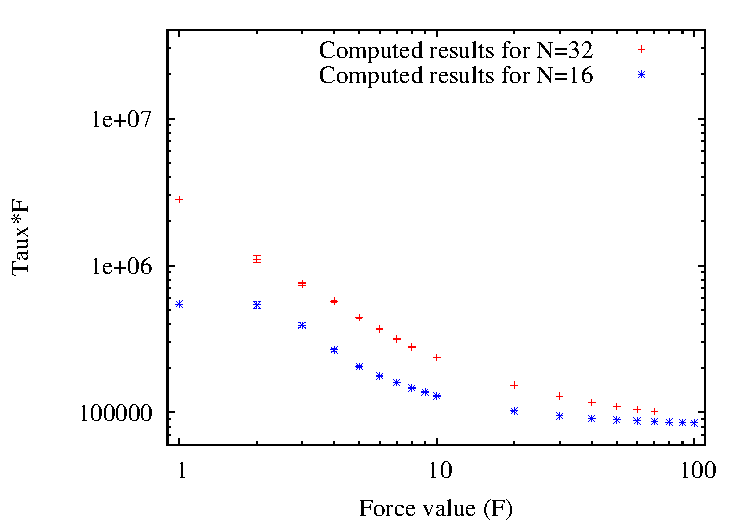
\includegraphics[width=0.5\textwidth]{translocvibf.pdf}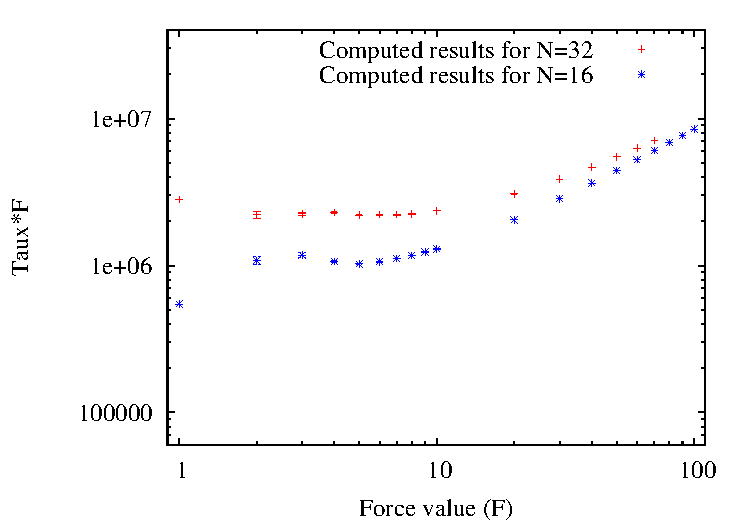
\includegraphics[width=0.5\textwidth]{translocvib.pdf}

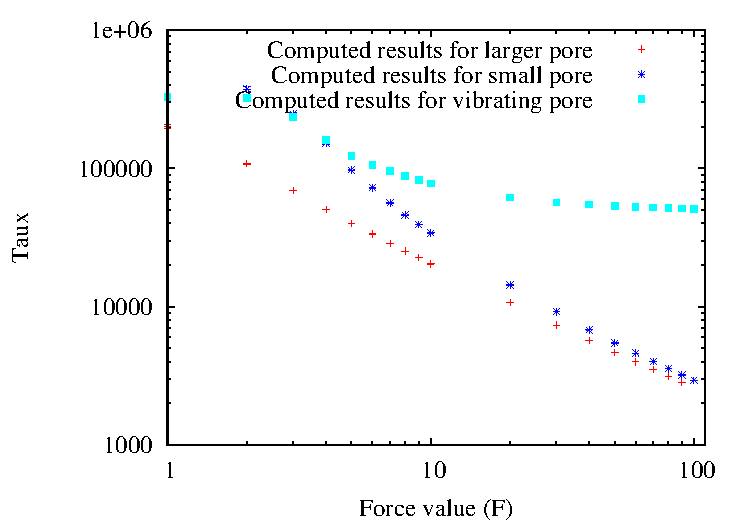
\includegraphics[width=0.5\textwidth]{translocporedifnbackup.pdf}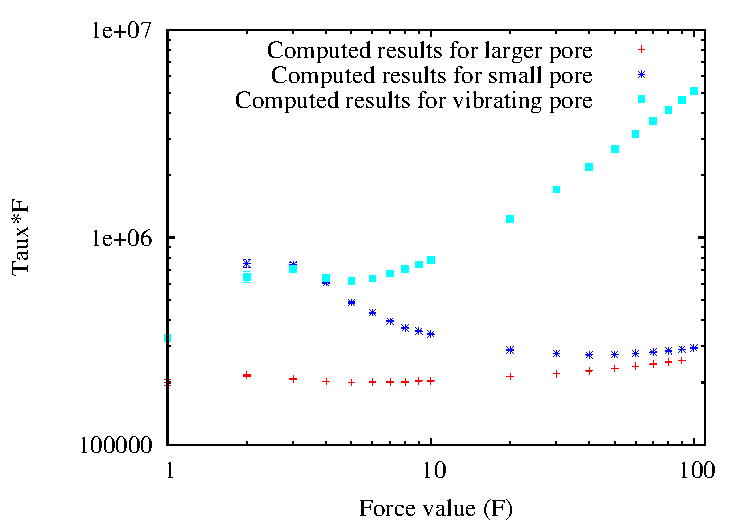
\includegraphics[width=0.5\textwidth]{translocporedifbackup.pdf}
\caption{Lors de l'étude de l'influence des vibrations, le temps de calcul est devenu significativement plus élevé. Les points sont pris pour seulement 150 translocation contrairement aux 1000 des cas précédents. Il a tout de même fallut trois semaines de calculs pour obtenir ces graphes. La partie gauche des courbes semble plausible, mais à forte forces, le temps de translocation semble saturer. Ces résultats semblent trop peu fiables pour que nous nous aventurions à les comparer avec les précédents.}
\label{surprise}
\end{center}
\end{figure}








\end{document}

